\RequirePackage[hyphens]{url} %fixes overflowing url-s in footnotes
\documentclass[en-lang,rdf-logo]{cyber-technical}
\usepackage[utf8]{inputenc}
\usepackage{hyperref}
\usepackage{scrextend}
\addtokomafont{labelinglabel}{\bfseries}

% Document metadata
\CyberDefineDocumentNumber{T-176-1}
\CyberDefineDocumentVersion{1.3}
\CyberDefineDocumentSecurity{}
\CyberDefineBackofTitlePage{\copyright\ Cybernetica, \the\year}
\CyberDefineCopyrightFooter{}

\setcounter{secnumdepth}{3}

\newcommand{\todo}[1]{\textbf{[TODO: #1]}}
\newcommand{\research}[1]{\textbf{[Further research needed: #1]}}
\newcommand{\discuss}[1]{\textbf{[Has to be discussed: #1]}}
\newcommand{\remark}[1]{\textbf{[Remark: #1]}}


\begin{document}

	\title{Analysis of planned architectural changes in Open-eID}

	\maketitle

~

\vfill

\begin{tabular}{ll}
Project leaders:		& Tõnis Reimo (Estonian Information System Authority)\\
						& Sandhra-Mirella Valdma (Cybernetica)\\
Contributing authors: 	& Kristjan Krips (Cybernetica)\\
						& Mart Oruaas (Cybernetica)\\
						& Alisa Pankova (Cybernetica)\\
						& Jan Willemson (Cybernetica)\\
\end{tabular}

Estonian Information System Authority, Pärnu maantee 139a, 15169 Tallinn, Estonia.\\
Email: \href{mailto:ria@ria.ee}{ria@ria.ee}, Web: \url{https://www.ria.ee},
Phone: +372 663 0200.

Cybernetica AS, Mäealuse 2/1, 12618 Tallinn, Estonia.\\
E-mail: \href{mailto:info@cyber.ee}{info@cyber.ee}, Web: \url{https://www.cyber.ee},
Phone: +372 639 7991.

\textcopyright~Estonian Information System Authority, 2020

\clearpage 

	\setcounter{tocdepth}{3}
	\tableofcontents{}

	\cleardoublepage

	\chapter{Executive summary}
Estonian State Information Agency (RIA) has initiated a process to update the ID-card (smart card) support in browsers to address various stability and support issues the current TLS client certificate authentication (CCA) based solution has. A team of researchers and developers has created an initial architecture draft for the new solution\footnote{\url{https://github.com/open-eid/browser-extensions2}}, which will be named Web eID. The purpose of the current document is to analyse this architecture from the security point of view.

To do this in a systematic way, we fixed the scope of the analysis, identified all the relevant digital assets present in the architecture, and considered possible actions an attacker could do (Create, Read/Use/Copy, Update, Delete) on them. As a result, this document lists the assumptions that the proposed solution relies on, along with the threats and mitigation measures.

The main scope of the analysis was limited to the components that are in the focus of development during the current project (server application, browser extension and Web eID native application). Note, however, that the full ecosystem is much wider, including the client and server platforms, trust service providers, browsers, etc. There are many potential threats emanating from them, and therefore it should be regularly reviewed if these threats are handled and whether additional mitigation measures should be implemented. 

The biggest change in the Web eID architecture compared to the previously used Open eID is the way how clients are authenticated. It is no longer possible to use client side authentication provided by TLS. While the change adds stability, it also affects the security of authentication. Not all configurations of the new Web eID architecture protect against man-in-the-middle attacks where the attacker is simultaneously able to do DNS-spoofing and provide a valid TLS certificate for client's browser.

Web eID was designed to allow the service provider to select between two protection profiles based on the level of acceptable risk. The first profile is easy to implement and protect, but is vulnerable to the aforementioned powerful man-in-the-middle attack. While in theory the stronger profile provides protection against powerful man-in-the-middle attacks during the authentication phase, it is non-trivial to implement. Currently only Mozilla's Firefox browser provides an API that allows to apply the second protection profile on the client side. Even if implemented, the limitations of browser API-s allow to protect only the authentication phase against the aforementioned man-in-the-middle attacks. Such attacks usually require a certificate authority to be compromised and are therefore unlikely to happen. However, the same risk applies to connections that are being legitimately monitored by corporate proxies.

As the majority of mainstream browsers are built on top of Google's Chromium, Google's representative was contacted in order to inquire about the possibility extend Chromium's API so that the aforementioned man-in-the-middle attacks could be avoided. The representative of Google responded that such measures are not in plan and are most likely not going to be implemented. One of the reasons is that a significant percentage of web traffic goes through corporate middleboxes\footnote{\url{https://blog.cloudflare.com/monsters-in-the-middleboxes/}}, which need to perform man-in-the-middle interception in order to scan traffic~\cite{DBLP:conf/ndss/DurumericMSBSBB17}. Corporate scanning of TLS traffic falls under the class of powerful man-in-the-middle attacks and thus affects Web eID. Therefore, corporate proxies become a single point of failure for Web eID in case the second protection profile is not implemented. An attacker or a compromised employee abusing the corporate proxy can intercept the session tokens and can replace the hash values that are being sent to be digitally signed by the client.

The second downside of the new architecture compared to TLS-CCA lies in the difficulty of preventing session hijacking attacks. TLS-CCA based architecture makes it possible to prevent session hijacking (i.e., copying of session identifiers), but there is no straightforward way to do that in the new architecture. This is a common problem, which is present in most of the mainstream authentication technologies as described in Section~\ref{sec:session_hijacking}. This can be a problem in the following cases:
\begin{itemize}
 \item a vulnerability in the web service or browser gives access to session identifiers,
 \item an attacker has temporary local access and can copy the session identifier,
 \item when HTTPS interception (proxy or middlebox) is used to monitor or mediate the traffic, the session identifier may leak.
 \end{itemize}

	\chapter{Introduction}

\section{Terminology}
\begin{itemize}

\item Browser extension -- third party code that is integrated with the browser API-s.

\item Certificate -- a file that binds the public key with the identity of the key owner. In this document, we are only considering certificates that are issued by certificate authorities.

\item Certificate authority (CA) -- a trusted third party, who issues certificates to end users (citizens or organisations) or assigns trust to lower level certificate authorities.

\item eID -- electronic identification, a digital solution for proof of identity of citizens or organisations.

\item Local attacker -- an attacker who has either physical or remote access to the user's computer.

\item Local attacker with administrative permissions -- an attacker who can do everything that the administrator can do. Such an attacker can be considered to control the whole computer, including what is displayed on the screen.

\item Local attacker with user permissions -- an attacker who does not have access to functionalities that require administrative permissions. Such an attacker can perform unprivileged system calls, which can differ depending on the operating system.

\item Man-in-the-middle attack (MITM) -- an attack where the attacker relays messages between two parties. Thus an attacker can eavesdrop and modify the exchanged messages.

\item Powerful attacker -- an attacker who can get a valid certificate for a selected domain and who is also able to perform DNS spoofing. This would enable running a man-in-the-middle attack.

\item Service provider -- the party who is running the web service / server application that provides the option for the client to authenticate or issue digital signatures by using the new browser extension.

\item TLS -- Transport Layer Security, a cryptographic protocol for secure Internet communication.

\item OCSP -- Online Certificate Status Protocol, an Internet protocol used for obtaining the revocation status of a X.509 digital certificate.

\item Web service -- the service which the client is authenticating to or which asks the client to give a digital signature with the Web eID browser extension.


\end{itemize}

\section{The scope of the analysis}
\label{sec:scope}
The new browser extension allows the web services to authenticate users and ask them to issue signatures. Thus, the main scope of the analysis contains the browser, native Web eID application, the service provider and their interaction (see Figure~\ref{fig:scope}).

\begin{figure}[ht]
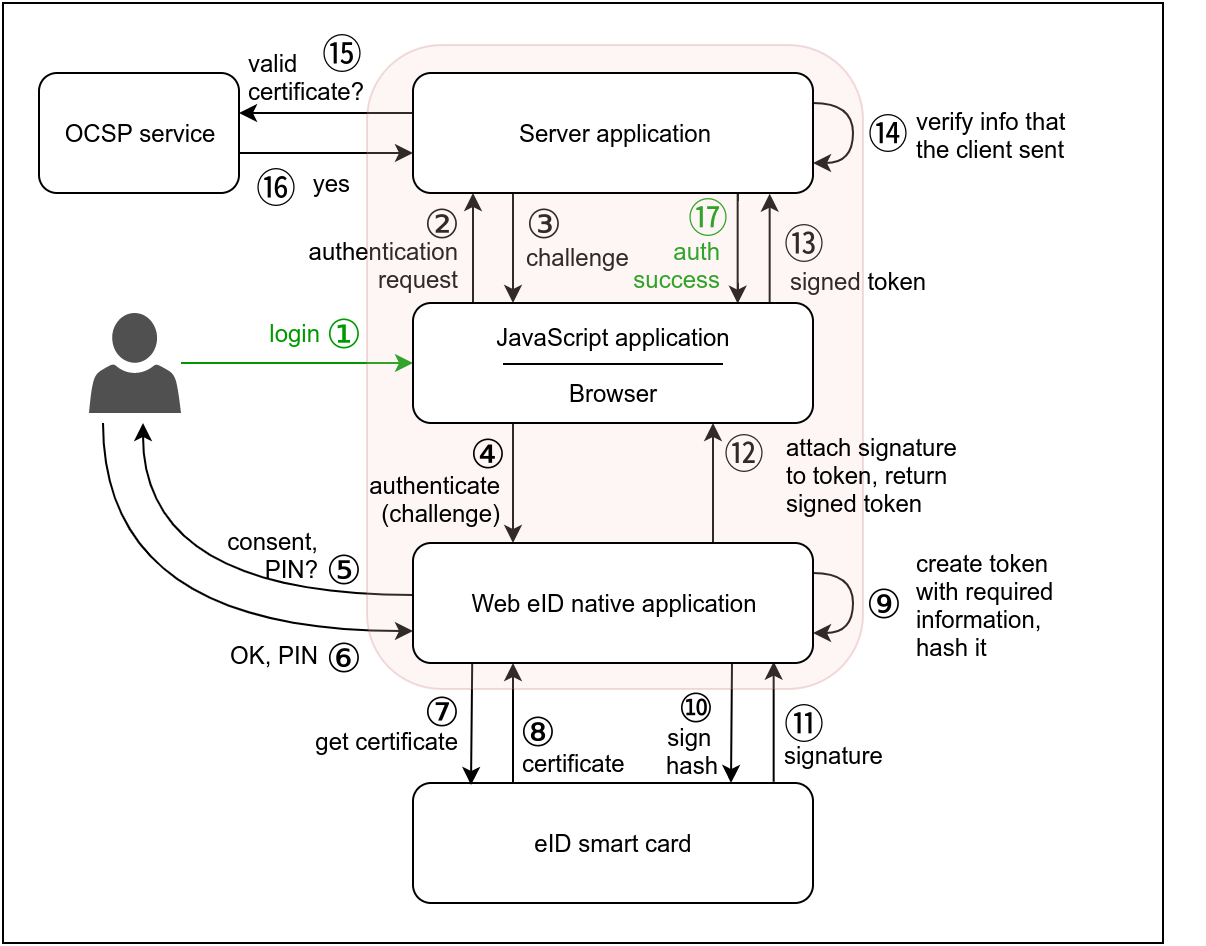
\includegraphics[width=\columnwidth]{img/main_scope_1.png}
\caption{The main scope of the current analysis is highlighted and covers the interaction between the server application, browser and native Web eID application. The  authentication and signing protocols are described in the  Web eID architecture draft: \url{https://github.com/open-eid/browser-extensions2}.}
\label{fig:scope}
\end{figure}

However, security of the new architecture also depends on multiple external factors that are not in the main scope, so at times we also need to talk about the extended scope.

For example, the user's device has to be trusted to behave correctly. It is difficult to protect user's digital identity while the device is infected and controlled by malware. Therefore, protecting user environment is mostly the responsibility of the user or the corresponding organisation. Although there are technologies that can protect the user in a malicious environment, they usually rely on additional hardware. Providing additional hardware for the end users is out of the scope of this project. Still, it may also be possible to apply software based mitigation measures to make it more difficult to attack the user environment. For example, an attack is more difficult if it requires superuser permissions.

In addition, the certificate authorities that issue eID certificates and TLS certificates for web services have to be trusted. The CA has to protect its signing key from third parties to prevent it being misused to issue fraudulent certificates. The CA also has to properly authenticate the party who is requesting a certificate. There are specific requirements which the certificate authorities have to follow. The security of the CA-s is out of the scope of this project. Thus, we assume that the certificate authorities behave according to their requirements and that they are properly audited.

Although the main scope of this analysis does not cover the CA-s and the local computer, the approach that we chose for the analysis tries to list all the relevant threats that could affect the security of authentication or signing in the new architecture. Therefore, we also list threats caused by entities that are out of scope of the Web eID architecture. Based on this information, the overall threat landscape can be seen. While the mitigation of external threats is not in the scope of this project, these threats could be mitigated by organisational measures or by third parties who are responsible for the corresponding components.

We recommend to conduct a follow-up study to investigate the threats to the end user from an untrusted computing device. It is important to understand how a compromised local machine can be abused depending on which level of access the attacker has to the system. As different operating systems have different API-s and permission systems, this study should be performed for each supported operating system.

\section{Security objectives and requirements}

\subsection{Security of authentication}

On a high level, authentication protocols need to achieve the following properties to be considered secure~\cite{BoMa10}.

\begin{labeling}{Entity authentication:}
    \item[Entity authentication:] the service provider obtains a reasonable level of assurance that the entity requesting authentication is who they claim to be.
    \item[Freshness:] the service provider obtains a reasonable level of assurance that the authentication request is recent.
\end{labeling}

Typically, we want the authentication to be \emph{mutual}, i.e. we also require the following property.

\begin{labeling}{Origin authentication:}
    \item[Origin authentication:] the user obtains a reasonable level of assurance that the service he/she is authenticating to is who they claim to be.
\end{labeling}

In order to satisfy these requirements, several lower level properties must hold.

\begin{labeling}{Impersonation resistance:}
    \item[Credential validity:] it must be possible to establish whether the credentials used for authentication are valid.
    \item[Authorised usage:] it must be hard to use the credentials in an unauthorised manner.
    \item[Impersonation resistance:] the protocol should provide reasonable level of assurance against malicious impersonation attacks (e.g. man-in-the-middle and session hijacking). 
    \item[Cryptographic strength:] the algorithms in use must withstand the attempts to violate the cryptographic properties. 
\end{labeling}

\subsection{Security of signing}

On a high level, signature protocols need to achieve the following properties to be considered secure.

\begin{labeling}{Entity authentication:}
    \item[Entity authentication:] the signature should identify the signing person/entity with high level of assurance.
    \item[Non-repudiation:] the entity who has given the signature is unable to deny neither the fact of signing, nor the knowledge of the signed content (together with all its possible binding implications) after the fact. 
    \item[Data integrity:] the party verifying the signature gets assurance that the data under the signature has not been changed between the moments of signing and verification.
\end{labeling}

In order to satisfy these requirements, several lower level properties must hold.

\begin{labeling}{Cryptographic strength:}
    \item[Credential validity:] it must be possible to establish whether the credentials used for signing were valid at the time of signing.
    \item[Authorised usage:] it must be hard to use the credentials in an unauthorised manner.
    \item[Cryptographic strength:] the algorithms in use must withstand the attempts to violate the cryptographic properties.
\end{labeling}


	\chapter{Technologies}

This chapter takes a look at the technologies used, criteria of choosing them and how they help to mitigate the threats identified in this report.

\section{Arguments for choosing OpenID Connect ID Token format and custom protocol}

Web eID has chosen OpenID X509 ID Token and a custom protocol as means of communicating the authentication result. The obvious alternative to the chosen protocol would be full WebAuthn support, but there are strong arguments against it:

\begin{enumerate}
    \item WebAuthn is overly complicated and not practical to implement for small e-service providers. Support by different web application frameworks is not (yet) sufficient.
    \item Specification is long (167 pages) and requires deep understanding of the technology, yet its first mentioned audience is "Relying Party web application developers". This does not sound viable, as Relying Party web application developers cannot be expected to be experts of such protocols, except in large organisations.
    \item It uses public key as end user identifier (not identifiers bound via PKI certificates) and is built around the "key pair per service" model. Using the same ID card key for all services may have strange implications (requires further analysis).
    \item The previous point also means that replacing an ID-card (and thus the keys) may have strange implications and may cause user lock-outs.
    \item It requires device attestation. Even though this can be skipped, device attestation does not conceptually apply to the eID ecosystem.
\end{enumerate}

Based on that, OpenID X509 ID Token is the superior option:

\begin{enumerate}
    \item It is based on a standard container format, offering digital signatures, symmetric integrity protection and authenticated encryption.
    \item It offers hypothetical future compatibility with OpenID Connect, or at least offers a cheaper migration path, as that technology is already known for e-service developers.
\end{enumerate}


\section{Token Binding}
\label{sec:token_binding}
Token Binding is a proposed extension for TLS using a key pair also on client's side of the connection\footnote{\url{https://tools.ietf.org/html/rfc8471}}, thereby being similar to TLS-CCA. Token Binding prevents strong man-in-the-middle attacks in cases where an attacker has access to a valid certificate for the target domain. In addition, it prevents session tokens or session cookies from being reused in another TLS session, thereby effectively preventing session hijacking attacks. This is achieved by cryptographically binding the session identifier to the randomness used in the corresponding TLS session. More specifically, the exported keying material (EKM)\footnote{\url{https://tools.ietf.org/html/rfc5705}} from the TLS session is signed by client's Token Binding key. 

When Token Binding is used together with TLS 1.2 (or older versions), then also the Extended Master Secret extension (RFC 7627)\footnote{\url{https://tools.ietf.org/html/rfc7627}} and TLS Renegotiation Indication (RFC 5746)\footnote{\url{https://tools.ietf.org/html/rfc5746}} extension must be used\footnote{\url{https://tools.ietf.org/html/rfc8471\#section-4.2}}.

One downside of Token Binding is that it would make it difficult to debug and monitor connections as HTTPS interception would break. Other concerns like using Token Binding for DRM can be found from Google's discussion boards\footnote{\url{https://groups.google.com/a/chromium.org/forum/\#!msg/blink-dev/OkdLUyYmY1E/w2ESAeshBgAJ}}\footnote{\url{https://groups.google.com/a/chromium.org/forum/\#!msg/blink-dev/r4zE8RKB6l4/0VNjdZRQAAAJ}}. Such concerns resulted in Google Chrome dropping the support for Token Binding in 2018. From the mainstream browsers it is only supported by Edge\footnote{\url{https://docs.microsoft.com/en-us/windows-server/security/token-binding/introducing-token-binding}}. However, the work on the Token Binding standard is continuing.

It is difficult to build a public service on top of Token Binding until it is not supported by mainstream browsers. Thus, alternative technologies should be used to provide similar protective measures. For example, Certificate Transparency is a technology that allows to detect powerful man-in-the-middle attacks.


\section{Certificate Transparency}
\label{sec:certificate_transparency}
Certificate Transparency (CT)\footnote{\url{https://tools.ietf.org/html/rfc6962}} is a protocol that is designed to limit the amount of damage from mistakenly or maliciously issued certificates. It works by creating public append-only logs of CA issued certificates, which allows to publicly monitor and audit new certificates. Thereby, the domain owner and the CA can monitor the logs and detect if a new (malicious) certificate is issued for a given domain.

Google Chrome started to enforce CT for new (public) certificates that were issued since April 30th  2018.\footnote{\url{https://groups.google.com/a/chromium.org/forum/\#!msg/ct-policy/wHILiYf31DE/iMFmpMEkAQAJ}} Certificates that were issued before that date got an exception and can still be used. However, in case a new certificate is issued without the support for CT, visiting the corresponding web site with Google Chrome results in a full page error with the code \texttt{net::ERR\_CERTIFICATE\_TRANSPARENCY\_REQUIRED}. Thus, in order for a website to be compatible with Google Chrome it has to comply with CT. As Google Chrome has the largest market share\footnote{\url{https://gs.statcounter.com/browser-market-share}}, it is inevitable that CT will be supported by almost all websites, which use TLS. In addition to Google Chrome, Safari also started to enforce CT for the certificates issued since October 15th  2018.\footnote{\url{https://support.apple.com/en-us/HT205280}} In 2019, a study was performed to measure the adaption and error rate of CT~\cite{DBLP:conf/sp/StarkSMOMFMT19}. Telemetry from Google Chrome was used in that study and it showed that in the beginning of February 2018, 71.1\% of requests for which CT would apply were CT-compliant. The study reported that by September 2018, CT-compliance was required for 42.6\% of connections and out of these 99.7\% of HTTPS requests were CT-compliant\footnote{\url{https://www.ieee-security.org/TC/SP2019/SP19-Slides-pdfs/Emily_Stark_-_3-Emily_Stark-Does_Certificate_Transparency_Break_the_Web-_Measuring_Adoption_and_Error_Rate_(1).pdf}}.

Service providers can force supporting browsers to strictly follow CT by using \texttt{Expect-CT} header\footnote {\url{https://developer.mozilla.org/en-US/docs/Web/HTTP/Headers/Expect-CT}}. For example, Google Chrome can be forced to follow CT also for certificates that were issued before April 30th 2018 by using \texttt{Expect-CT} header. That way it is possible to prevent attacks with certificates that were issued before April 30th 2018.

One open issue with CT is its support by other browsers. Until all major browsers will start to enforce CT, it can not prevent targeted attacks. The other issue is that the service providers and the CA-s have to be active to monitor and detect maliciously issued certificates so that they could be revoked in time.

One way how CT can be implemented is by using OCSP stapling (see Section~\ref{sec:ocsp_stapling}). However, the main benefit of using OCSP stapling is to make sure that information about certificate revocation is sent to the client's browser.


\section{OCSP stapling}
\label{sec:ocsp_stapling}
OCSP is used to check whether a given certificate is valid at a given time point. However, there are multiple problems with client side OCSP queries, one of them being the leakage of private information regarding the web sites the client is using.

OCSP queries are relevant in the new architecture in two ways. First one is explicitly illustrated in Figure~\ref{fig:scope} where the service provider checks if the client certificate is valid. Second, the client can also check whether the service provider's certificate is valid while initiating the TLS connection (however, some browsers skip the OCSP queries).

The validity check for the service provider's certificate is required to avoid man-in-the-middle attacks in case service provider's private key has leaked. However, currently browsers use soft fail in case OCSP service is briefly unavailable or the query is blocked. In these cases browsers proceed with the TLS connection, although OCSP response is missing. Therefore, by performing client side OCSP queries, the client can not get the guarantee that the certificate of the web site is valid. In addition, client side OCSP requests violate privacy of the user as the OCSP provider will find out when and which web sites the corresponding client visits.

The solution to both of these issues is to use OCSP stapling\footnote{\url{https://tools.ietf.org/html/draft-hallambaker-tlsfeature-05}}. This allows the service providers to deliver the OCSP response to the client together with the TLS certificate. To prevent downgrade attacks, this functionality must be enforced by setting OCSP Must-Staple flag in the certificate. This functionality is independent of the Web eID architecture and has to be separately configured by the service provider. Although OCSP stapling may seem to be out of scope regarding the new architecture, it is actually relevant to protect the end users against man-in-the-middle attacks.

Just relying on OCSP stapling and Certificate Transparency is not sufficient to prevent man-in-the-middle attacks as they are not yet universally supported. Thus, Web eID architecture contains its own mitigation measures to prevent man-in-the-middle attacks as described in Section~\ref{sec:cert_validation}. However, these measures do not fully eliminate the threat from man-in-the-middle attacks as client's session can span multiple TLS sessions as described in Section~\ref{sec:tls_resumption}.


\section{TLS session resumption}
\label{sec:tls_resumption}
The proposed Web eID browser extension architecture allows to use multiple TLS connections in the same authenticated session. For example in Section~\ref{sec:cert_validation} it is described that during the authentication phase two different TLS connections are used to make queries to the service provider. A new TLS session could also be initiated when the client temporarily loses Internet connection, however, this does not invalidate the authenticated session.

Therefore, MITM protection should be provided not only for the initial authentication query, but also for negotiating a new TLS session. This is a non-trivial functionality, which is not implemented in the first version of Web eID. The reasoning for that is given in Section~\ref{sec:mitm_risks_mitigations}.

One possible solution to this problem is to rely on TLS session resumption and force re-authentication when resumption is rejected. Whether this approach could be applied in practice depends on the server side architecture, i.e., whether the information about TLS session resumption is available to the web service.

In the following we consider only TLS 1.2 and TLS 1.3 as mainstream browsers will end the support for TLS 1.0 and TLS 1.1 for regular users in the beginning of 2020.\footnote{\url{https://blog.mozilla.org/security/2018/10/15/removing-old-versions-of-tls/}}\footnote{\url{https://blogs.windows.com/msedgedev/2018/10/15/modernizing-tls-edge-ie11/}}\footnote{\url{https://webkit.org/blog/8462/deprecation-of-legacy-tls-1-0-and-1-1-versions/}}

TLS resumption in TLS 1.2 is provided either by SESSION ID (RFC 5246)\footnote{\url{https://tools.ietf.org/html/rfc5246\#appendix-F.1.4}} or by SESSION tickets (RFC 5077)\footnote{\url{https://tools.ietf.org/html/rfc5077}}. TLS 1.3 replaces these with resumption based on pre-shared keys (RFC 8446)\footnote{\url{https://tools.ietf.org/html/rfc8446\#page-15}}.

However, in order to prevent MITM during TLS resumption, the extended master secret extension (RFC 7627\footnote{\url{https://tools.ietf.org/html/rfc7627}}) must be used. This extension ties the master secret to the hash of the messages sent during the handshake. Thus, it prevents MITM that would negotiate two TLS sessions with the same master secret.

	\chapter{Compatibility with TLS Client Certificate Authentication}
\label{chapter:TLS-CCA}
TLS Client Certificate Authentication (CCA) provides mutual authentication and thereby gives some additional security guarantees compared to one-way TLS, where only the server is authenticated. Below follows a list of some of the relevant properties and security features that may be offered by TLS-CCA:

\begin{itemize}
\item In the case of mutual authentication, the client signs all previous handshake messages that were exchanged during TLS session negotiation. The signed result is delivered to the server in the \texttt{CertificateVerify} message. Thus, the signature covers, among other things, the randomness selected by the server, randomness selected by the client, the server's certificate and the encrypted pre-master secret that the client chose\footnote{\url{https://tools.ietf.org/html/rfc5246}}.

	\begin{itemize}
	\item Client can not be successfully manipulated by a man-in-the-middle attack even when the middleman has obtained a fraudulent certificate for a service provider as the server's certificate and pre-master key are signed by the client.

	\item It would still be possible for the middleman to successfully interact with the client, however, in this case the messages could not be relayed to the real server.
	\end{itemize}

\item TLS-CCA allows to bind the whole session to client's certificate if TLS-CCA is forced also after the login phase. This requires the service provider to request authentication for each request. However, this forces keeping the authentication security context activated on the ID-card in Open eID architecture after initial PIN1 entry, which poses a security threat of its own (otherwise the user would be required to enter PIN1 for every new HTTPS request, including requests for page assets like images and scripts, which would not be feasible).

	\begin{itemize}
	\item It gives protection against session hijacking. E.g., phishing or using XSS to steal a session cookie becomes irrelevant as a third party can not use the cookie.
	\end{itemize}
\end{itemize}


\section{Comparison of TLS-CCA with other common authentication architectures}
Many authentication systems are using signed tokens. However, in case the token is not bound to the TLS session, it is not possible to prevent an attacker from using a leaked session identifier. In such systems, session hijacking can not be prevented once the session identifier leaks. TLS-CCA-based Open eID is an exceptional case which, when configured correctly, can prevent session hijacking even when a valid session identifier leaks. However, the Web eID architecture along with other commonly used authentication systems like OpenID Connect, Mobile-ID, Smart-ID and WebAuthn (without Token Binding) is not able to prevent the session token from being reused in a different machine in case the session identifier leaks. Therefore, the threat of session hijacking must be mitigated by taking other measures against session identifier leakage.

To prevent MITM attacks, the other communication party has to be authenticated. TLS-CCA is based on mutual authentication and, when configured correctly, prevents MITM attacks. In case of Web eID, the service provider can decide how well the authentication phase is protected against MITM attacks. Based on that decision either origin validation or certificate validation can be applied, which are described in Sections~\ref{sec:origin_validation} and \ref{sec:cert_validation}. However, the MITM protection only applies to the authentication phase. The following TLS sessions which reuse the same session identifier are not protected against MITM attacks. The same observation holds true for other authentication systems which do not re-authenticate new TLS sessions after the initial client authentication. Still, neither the TLS-CCA based Open eID architecture nor the Web eID architecture can stop an attacker who has obtained a proper domain certificate from successfully interacting with the client. However, Certificate Transparency can mitigate such attacks, along with most MITM attacks against TLS regardless of the used architecture.

Client's private key is usually protected with a second authentication factor which unlocks the access to it. In the case of Open eID, Web eID, Mobile-ID and Smart-ID, access to the private key operations is restricted by requiring a PIN code. However, there is no straightforward mechanism to prevent the PIN code from being read in case malware has infected the corresponding device. Although in case of Open eID and Web eID it is possible to use card readers with a dedicated PIN-pad, such readers are not currently available on the local market and there are very limited options to get such hardware from the global market.

In case user's device is controlled by malware, the question arises whether the malware can use the authentication or signing functionalities without user interaction. When access to the private key operations is protected with a PIN code, the question is whether the malware is able to use the corresponding API without the user interaction. This is not possible when ID card is used with a PIN-firewalled PIN-pad-based reader. But when the smart card is directly connected to the infected device, the answer is not straightforward and depends on the local API-s and of the operating system in use. Thus, we give a recommendation in Section~\ref{rec:modeling-runtime-environment} to further study such issues.



\section{Session hijacking attacks}
\label{sec:session_hijacking}
The session identifier acts as a shared secret between the client and the service provider so that the service provider can link the user to the session. Thus, after a successful authentication, the user is assigned a session identifier. As usually the user is authenticated once during the session, it is assumed that the protective measures are sufficient to protect the session identifier from being leaked during an active session. However, when an attacker can somehow access an active session identifier, it can lead to a session hijacking attack.

Session hijacking is an attack which allows an attacker to access the victim's active session by reusing the captured session identifier (e.g., cookie, token), which is linked to the victim. Once the attacker has obtained access to the session identifier, it is difficult to prevent the attack as most of the mainstream authentication protocols/standards do not offer protection against session hijacking. 

In order to prevent session hijacking, the service provider would have to be able to verify the identity of the client by other means besides the session identifier. The standard approach is to use public key cryptography by asking the client to prove that it can use its secret key. The other approaches like matching client's IP and user agent, or frequently changing session identifiers are hacks, which are used to make the attack more difficult\footnote{\url{https://cheatsheetseries.owasp.org/cheatsheets/Session\_Management\_Cheat\_Sheet.html\#binding-the-session-id-to-other-user-properties}}. 

The two well known technologies, which use public key cryptography to prevent session hijacking attacks, are TLS-CCA, which is described in the beginning of Chapter~\ref{chapter:TLS-CCA}, and Token Binding, which is briefly described in Section~\ref{sec:token_binding}. Other authentication technologies like Mobile-ID\footnote{\url{https://www.id.ee/index.php?id=36881}}, Smart-ID\footnote{\url{https://www.smart-id.com/}}, PIN-calculator (passcode device / security token), or OpenID Connect are only used during the authentication phase, and after that the session identifier is usually protected by TLS. WebAuthn\footnote{\url{https://www.w3.org/TR/webauthn/}} and FIDO2 can prevent the session hijacking attacks when used together with Token Binding\footnote{\url{https://fidoalliance.org/fido-technote-the-growing-role-of-token-binding/}}. However, Token Binding is currently not supported by any of the mainstream browsers as discussed in Section~\ref{sec:token_binding}. Therefore, TLS-CCA is currently the only mainstream technology that provides sufficient protection against session hijacking.

Although the mainstream authentication technologies do not prevent session hijacking on their own, the threat can be mitigated in most cases (except for a targeted attack) by using proper configuration and security measures to prevent the leakage of the session identifier. There are four main ways for accessing the session identifiers:
\begin{itemize}
	\item malware on victim's device,
	\item cross-site scripting vulnerability on the service provider's web site, 
	\item session fixation vulnerability, 
	\item vulnerability which allows to intercept the traffic that contains the session identifier.
\end{itemize}
To prevent session fixation, the service provider has to update the session identifier after the user has authenticated. The session identifier has to be sufficiently random to prevent it from being guessed. The session identifier must be transported between the client and the server over a channel that is protected by TLS. However, the used TLS version and configuration also affect the security. The service provider's web site must have protective measures that prevent cross-site scripting attacks by properly escaping and encoding user input. Building such functionality is non-trivial, and thus it is usually provided by the framework which is used to build the web site. However, the protective measures are not necessarily active by default, and thus may need to be manually switched on. To offer additional protection against cross-site scripting and other common vulnerabilities, the session cookie has to have the following flags: HttpOnly, Secure, SameSite\footnote{\url{https://cheatsheetseries.owasp.org/cheatsheets/Session_Management_Cheat_Sheet.htm\#security-risks}}. Unfortunately, the service provider can not protect user's session in case user's device is infected by malware.






\chapter{Protection against man-in-the-middle attacks}\label{sec:protection_profiles}
The proposed architecture specifies two ways of how the service provider can configure the protection against man-in-the-middle attacks. The simpler method, which is briefly described in Section~\ref{sec:origin_validation} is based on origin validation and is therefore easy to implement, but this comes with a higher risk for an attack. Origin validation does not protect against powerful man-in-the-middle attacks where the attacker is simultaneously able to do DNS-spoofing and provide a valid TLS certificate for client's browser.

The alternative method, which is described in Section~\ref{sec:cert_validation} forces the client to sign the service provider's certificate, thereby allowing the service provider to detect interference in case a wrong certificate is signed by the client. While in theory the certificate validation based method provides protection against powerful man-in-the-middle attacks during the authentication phase, it is non-trivial to implement and can currently be used only with Firefox. 

We also describe a third approach in Section~\ref{sec:challenge_signing}, which is based on the service provider signing the challenge, but this method is not implemented in the new architecture. Regardless of the chosen architecture, some risks regarding MITM attacks remain. These are described in Section~\ref{sec:mitm_risks_mitigations} along with possible mitigation measures.

Therefore, the service provider should make the choice of the protective measures based on a risk analysis.

\section{Origin validation}
\label{sec:origin_validation}
The origin validation architecture is based on WebAuthn\footnote{\url{https://www.w3.org/TR/webauthn-1/}} authentication process. In WebAuthn, the client has to sign the challenge sent by the web service along with the origin, i.e., the hostname of the web service. Thus, a man-in-the-middle attack should be prevented by the web service who checks that the correct origin is signed by the client.

However, an attacker who has access to a maliciously issued certificate for the given web service and is also able to perform DNS spoofing can easily bypass origin validation. Such attacks usually require a certificate authority to be compromised and are therefore unlikely to happen. However, the same risk applies to connections that are being legitimately monitored by corporate proxies. With such an attack the whole authenticated session is vulnerable and the corresponding communication can be intercepted and modified by the attacker. The attack could be initiated for any new TLS session negotiation in order to capture the session identifier that was previously created when the client authenticated to the web service. In addition, the malcious man-in-the-middle attacker could replace the hash value that is being sent to be digitally signed by the client browser, thereby creating a risk for the client to blindly issue a digital signature.

As mentioned previously, the probability of a certificate authority being compromised is low. However, the main risk comes from local man-in-the-middle attacks as origin validation does not detect and prevent a local MITM done by a middlebox, antivirus or malware. Therefore, in case of origin validation, corporate proxies become a single point of failure. An attacker or a compromised employee abusing the corporate proxy can intercept the session tokens and can replace the hash values that are being sent to be digitally signed by the client. 

It is important to note that Certificate Transparency may not apply to locally issued certificates as it is in the case of Google Chrome\footnote{\url{https://groups.google.com/a/chromium.org/forum/\#!msg/ct-policy/wHILiYf31DE/iMFmpMEkAQAJ}}. Thus, it is possible to debug origin validation based architecture with a MITM based testing tool like Burp Suite\footnote{\url{https://portswigger.net/burp}}.

Although the threat of man-in-the-middle attack is not fully mitigated, the approach may be sufficient for web services that do not require the highest level of security. In addition, the threat can be partially mitigated by relying on Certificate Transparency.


\section{Certificate validation}
\label{sec:cert_validation}
The certificate validation architecture takes origin validation as a basis and adds protection against powerful man-in-the-middle attacks where the attacker is simultaneously able to do DNS-spoofing and provide a valid TLS certificate for client's browser. With this approach the client signs the challenge, origin and the fingerprint of the certificate of the corresponding web service.

The web service must check if the signed information received from the client contains the correct certificate fingerprint. In case it does, the client used the correct certificate to establish the TLS connection. When the signed fingerprint does not match, the server has detected an attack and aborts the connection.

The difficulty with this approach lays in proxies which terminate the TLS connection. Multiple TLS certificates may be available for a given domain. The web service has to get access to the correct TLS certificate in order to verify the certificate fingerprint. Thus, the service provider has to make sure that the certificate is both available and up to date to prevent self inflicted denial of service attack in case the TLS certificate is replaced.

This approach prevents the usage of local MITM by a middlebox, antivirus or malware during the authentication phase. Therefore, certificate validation based architecture offers protection against local interception, which offers higher level protection than mainstream authentication technologies. This measure can also be provided by certificate pinning or by using TLS-CCA. However, the downside is that the information exchanged during authentication phase can not be easily debugged with a MITM based testing tool like Burp Suite\footnote{\url{https://portswigger.net/burp}}.

While certificate validation based authentication protects against powerful MITM attacks, it does this only during the authentication phase. Even protecting the authentication queries is non-trivial as the browser extension uses two different TLS sessions to initiate the authentication and to deliver the signed response to the service provider. Thus, the extension has to check that the second TLS session is established with the same party. To do this, the extension has to store a reference to the previous certificate and check whether the server certificate in the second TLS connection matches the previously seen certificate. It is crucial that the certificate is validated before the signed challenge is sent out as otherwise the man-in-the-middle would get access to the session. Even when this problem is solved, the rest of the authenticated session is vulnerable to a MITM attack in case the same session identifier is reused in a new TLS connection.

Currently only Mozilla's Firefox provides an API that allows to apply the certificate validation based protection profile. As the majority of mainstream browsers are built on top of Google's Chromium, Google's representative was contacted in order to inquire about the possibility extend Chromium's API so that the aforementioned man-in-the-middle attacks could be avoided. The representative of Google responded that such measures are not in plan and are most likely not going to be implemented. One of the reasons is that a significant percentage of web traffic goes through corporate middleboxes\footnote{\url{https://blog.cloudflare.com/monsters-in-the-middleboxes/}}, which need to perform man-in-the-middle interception in order to scan traffic~\cite{DBLP:conf/ndss/DurumericMSBSBB17}.


\section{An alternative approach: signing the challenge}
\label{sec:challenge_signing}
MITM attack against the authentication phase could also be mitigated if the service provider would sign the challenge sent to the client. With this approach, the client must be able to verify that the signed challenge is either directly or indirectly connected with the TLS certificate. I.e., either the challenge is signed by the private key that corresponds to the certificate, or the private key of the certificate would be used to delegate trust to a new key pair. The idea is to bind the TLS certificate to the challenge and thereby prevent the MITM from forwarding a different certificate to the client. In case of a MITM attack, the service provider would be able to verify both signatures and detect an attack. As this approach requires more configuration from the service provider to make the private key associated with the TLS certificate available to the service, it is not implemented in the first version of the new architecture.


\section{Remaining risks and possible mitigations}
\label{sec:mitm_risks_mitigations}
As previously mentioned, the proposed architecture is not able to prevent MITM attacks in case a new TLS session is established after the authentication phase. While there are multiple options for mitigation, these approaches may not be practically feasible and are not guaranteed to work in all scenarios.

The simplest option is to rely on Certificate Transparency, which is briefly described in Section~\ref{sec:certificate_transparency}. However, Certificate Transparency is not yet supported by all mainstream browsers. Nevertheless, its preventive aspect deters attacks that scale. Still, targeted attacks can not be ruled out.

Certificate Authority Authorization (CAA) provides website owners a way to specify in a DNS record, which certificate authorities are allowed to issue certificates for the corresponding domain~\cite{rfc8659}. The usage of CAA should reduce the risk of certificate authorities accidentally issuing certificates for an attacker. However, it does not prevent targeted attacks in case a certificate authority is compromised.

In addition, the service provider may only allow one TLS session per authenticated session such that TLS resumption would be the backup option when the client loses connection. This approach is technically non-trivial to implement and may not be practical. More information about this approach can be found in Section~\ref{sec:tls_resumption}.

The fourth option would be to keep a local reference of the original TLS certificate used during the authentication phase in the Web eID browser extension. Thus, for each new TLS connection the fetched certificate should be matched with the previously stored certificate. Implementing this in practice is non-trivial, and therefore this approach will not implemented in the first version of the new browser extension. 

Currently only Firefox provides an API that allows to query information about the TLS session, including the used certificate\footnote{\url{https://developer.mozilla.org/en-US/docs/Mozilla/Add-ons/WebExtensions/API/webRequest/getSecurityInfo}}. To implement local MITM protection, access to such an API is crucial. However, testing the Firefox API revealed that the certificate information can be queried only after a request has already been sent. Thus, while the API allows to detect MITM attacks it can not prevent a request being sent out to the middleman. The implication is that the authentication token can be delivered before detecting the attack. This could be mitigated if the API would allow to cancel requests based on the queried TLS configuration. However, even detecting a MITM attack is a step forward. The issue does not create a significant new vulnerability as session hijacking is also possible after the authentication phase as mentioned in Section~\ref{sec:cert_validation}. Thus, to prevent session hijacking the whole authenticated session would have to be protected against it.

In addition, the service provider also has to make sure that its certificate is revoked in case the corresponding private key leaks. However, revoking by itself is not sufficient as the information also has to reach the client as otherwise MITM attack may become possible. Fortunately, OCSP stapling with the Must-Staple flag resolves this issue. This approach is described in Section~\ref{sec:ocsp_stapling}.

	\chapter{Threats and assumptions}

This chapter contains the analysis part of this document. We begin by describing the methodology used for the analysis. Then the system components relevant for the analysis are listed. Section~\ref{sec:threats} contains the list of threats that directly affect the Web eID architecture. Section~\ref{sec:out_of_scope_threats} lists the threats that are not in the scope of the Web eID architecture but which can affect its security. Finally, the chapter is concluded by Sections~\ref{sec:satisfiable_assumptions} and \ref{sec:unsatisfiable_assumptions}, which give an overview of the assumptions that were used in the analysis. These assumptions are classified into two categories, the first one describes the assumptions that can be satisfied with the current technology, and the second one the assumptions that can not be satisfied with the current technology.

To create the list of threats in a systematic way, we fixed the scope of the analysis, identified the relevant digital assets present in the Web eID architecture, and considered possible actions an attacker could do (Create, Read/Use/Copy, Update, Delete) on them. Based on that we created a list of threats that covers all possible combinations of assets and the actions the attacker could do on them. However, by using such methodology also the non-relevant threats are listed. Thus, some of the listed threats are not relevant for the architecture or are not in the main scope of this analysis. We still include them for the sake of completeness. In principle it would also be possible to classify the threats further by also including the location of the attacker. However, we decided not to do that as for most of the threats the location is fixed by the context. 


\section{System components}

\subsection{Assets}
The system has the following (digital) assets:
\begin{itemize}
\item client's authentication key (part of 1st key pair),
\item client's signing key (part of 2nd key pair),
\item client's certificate, containing public key from the ID-card (either from 1st or 2nd key pair),
\item client's certificate trust store (browser or OS based),
\item service provider's long term private key,
\item service provider's certificate, which is signed by a trusted CA,
\item eID CA's signing key, which was used to issue the certificates for the ID-card,
\item CA's signing key, which was used to issue the certificate for the service provider,
\item client's PIN1, which unlocks the authentication key,
\item client's PIN2, which unlocks the signing key,
\item data, which client intends to sign,
\item hash of the data, which client intends to sign,
\item signed hash of the data, which client intended to sign,
\item container, which contains signed data,
\item service provider's authentication challenge,
\item unsigned authentication token,
\item hash of the unsigned authentication token,
\item signed hash of the authentication token together with the authentication token,
\item OCSP response for the client certificate,
\item session cookie set by the service provider.
\end{itemize}


%\subsection{Subjects}


\subsection{Locations}
Events may take place in the following locations:
\begin{itemize}
\item service provider's server,
\item communication channel between end-user's browser and service provider's server,
\item end-user's browser,
\item channel between end-user's browser and Web eID native application controller component\footnote{\url{https://github.com/open-eid/browser-extensions2\#native-application}},
\item channels between application controller component and \emph{libgui}, \emph{libpcsc}, \emph{libeid} components,
\item communication channel, which is used to interface with the smart card,
\item firmware / driver of the smart card reader.
\end{itemize}


\subsection{Actions}
\begin{itemize}
	\item Create -- attacker manages to create a valid asset.
	\item Read, Use, Copy -- attacker gains read-only access to an asset.
	\item Update -- attacker (successfully) modifies an asset.
	\item Delete -- attacker removes an asset either from storage or from communication channel.
\end{itemize}


	\newpage
\section{Threats}
\label{sec:threats}


\subsection{Attacker reads/uses/copies a certificate.}
The certificate can not be successfully used for authentication and signing without having access to the corresponding private key.

The certificate itself can be considered to be public information. The TLS certificates of web sites are public. Although the ID-card certificates contain somewhat private information about the client these certificates can be publicly queried using the personal identification code. The signing certificate is also included in the digital signature container (e.g., BDOC, ASiC-E).

However, the client may not want to disclose her identity to the service provider. Thus, the user has to decide whether the certificate should be sent to the service provider once authentication is initiated. By bypassing this check the website could track the user without user's consent. In addition, the client certificate should be encrypted when it is sent to the server.

Possible mitigations:
\begin{itemize}
\item The project documentation states that the implementation must require the user to interact to choose whether to continue with the authentication process and share the certificate with the service provider\footnote{\url{https://github.com/open-eid/browser-extensions2}}.

\item The information in the client certificate can be protected by delivering the certificate only over a TLS channel. This is not done with TLS-CCA~\cite{DBLP:conf/ndss/Parsovs14}, as the client certificate is transmitted in cleartext during the TLS-CCA handshake. The new Web eID architecture solves this issue.
\end{itemize}

 



\subsection{Attacker creates a new certificate trust store for the client.}
\label{threat:create-trust-store}
For an attacker it is sufficient to add one trusted CA to the trust store to be able to impersonate the service provider. Thus, this threat is equivalent to the threat in Section~\ref{threat:update-trust-store}. The threat can partially be mitigated by using the certificate validation based MITM protection, which is described in Section~\ref{sec:cert_validation}.


\subsection{Attacker reads/uses/copies client's certificate trust store.}
\label{threat:read-trust-store}
The certificates in the trust store can be considered to be public. Thus, the attacker does not get an advantage by just getting read access to these certificates. 

\subsection{Attacker updates client's certificate trust store.}
\label{threat:update-trust-store}
By adding a root certificate to client's trust store the attacker will  be able to issue certificates, which are trusted by client's browser or operating system.

Thus, the attacker is able to impersonate any web service, which does not use pinned certificate or pinned public key. Therefore, with the help of DNS spoofing it is possible to run a man-in-the-middle attack against such web sites. It is important to understand that Certificate Transparency may not work for locally issued certificates as the functionality depends on browser configuration. For example, Google Chrome follows Certificate Transparency only for public certificates\footnote{\url{https://groups.google.com/a/chromium.org/forum/\#!msg/ct-policy/wHILiYf31DE/iMFmpMEkAQAJ}}. 

Possible mitigations:
\begin{itemize}
\item The service provider could theoretically use certificate or public key pinning as mitigation. However, it is difficult to implement pinning correctly and it may cause issues with stability. This is the reason why several browser vendors have removed support for HKPK\footnote{\url{https://www.chromestatus.com/feature/5903385005916160}}\footnote{\url{https://www.fxsitecompat.dev/en-CA/docs/2019/http-public-key-pinning-is-no-longer-supported/}}.

\item By forcing the client to sign the service provider's certificate fingerprint along with the challenge, the real service provider can detect a MITM attack during the authentication phase by comparing the signed certificate fingerprint with the fingerprint of its own certificate. More information about the certificate validation based MITM protection can be found from Section~\ref{sec:cert_validation}. This measure does not protect the session identifier against MITM attacks that are conducted after the authentication phase during a new TLS negotiation.
\end{itemize}


\subsection{Attacker deletes client's certificate trust store or parts of it.}
\label{threat:delete-trust-store}
In case a trusted root certificate is removed from the trust store, the client may not be able to visit web sites or use web services, which rely on that root certificate. Thus, such action can lead to a denial of service attack. However, the attack does not scale as it requires either remote or physical access to end-user's device.





\subsection{Attacker creates data, which is sent to be signed.}
\label{threat:create-data-for-signing}
It must not be possible to sign two different documents by issuing a digital signature for only one of these documents. During the signing process the hash of the document is signed and not the file itself. Therefore, it must not be possible to find two different documents that give the same hash value. This must be prevented by the design and choice of the corresponding hash function. 

Thus, we assume in this analysis that the attacker is not able to break the collision resistance property of the cryptographic hash function that is used for signing.

This threat is relevant both for authentication and signing as in both cases a value is sent to be signed with one of client's private keys. The attacker could either initiate the signing process on its own and trick the user into entering the PIN code or replace the data that the client intends to sign (see~\ref{threat:update-data-for-signing}). The service provider may also play the role of an attacker as it could display information that is different from the data that is going to be signed by the client. See, Section~\ref{threat:create-hash-for-signing} for more info.

Relevant locations: 
\begin{itemize}
\item Service provider
\item Communication channel
\item Client's browser
\item Client device's operating system
\end{itemize}

Possible mitigations:
\begin{itemize}
\item The integrity of the communication channel is protected by TLS.

\item The user should always be able to view what is being signed. This may prevent the malicious or compromised service provider from tricking the user into signing the data that was created by the attacker. 

\item The user should be able to download the signature as it can be later used as a legal proof in case of fraud. Without having the possibility to download and store the signed information the client has no basis to dispute the legality of the signature. 

\item An independent card reader with a trusted display could allow the client read and verify what is being signed.

\item A collision resistant cryptographic hash function must be used for signing.
\end{itemize}


\subsection{Attacker reads/uses/copies data, which is sent to be signed.}
\label{threat:read-data-for-signing}
For legally binding signatures this is generally not a threat as signing does not provide confidentiality. In case confidentiality is required, it has to be achieved with other measures like encryption.

For authentication, see~\ref{threat:read-authchallenge}. 


\subsection{Attacker updates data, which is sent to be signed.}
\label{threat:update-data-for-signing}
We assume in this analysis that the attacker is not able to break the collision resistance property of the cryptographic hash function that is used for signing. For more info, see~\ref{threat:create-data-for-signing}.

This threat is relevant both for authentication and signing as in both cases a value is sent to be signed with one of the private keys. Attacker's actions can be seen as a man-in-the-middle attack where the attacker replaces the initial value that the card owner wanted to sign. Such an attack works even in the case where PIN-pad is used and when the attacker does not have access to the PIN codes. The user is willing to enter the PIN-code to complete the current action and therefore does not expect to sign a different value. The attack can be hidden by showing an error which the users are quite used to, which in turn means that the attack might stay unnoticed.

In case of issuing a legally binding signature, this attack can lead to legal dispute as the attacker is able to decide what should be signed. The service provider may also play the role of an attacker as the service provider could display information that is different from the data that is going to be signed by the client. See, Section~\ref{threat:create-hash-for-signing} for more info.

In case of authentication, the attacker can replace the authentic challenge sent by one service provider with a challenge from another service provider in order to get access to the client's account, which is connected with the second service provider.

Locations for this attack:
\begin{itemize}
	\item A malicious service provider could  display to the client one value but may ask to sign a different value.
	\item Browser (e.g. using a malicious browser extension) can imitate the behaviour of a valid ID-card extension. In addition, currently it is not possible to limit the access that Google Chrome and Firefox extensions have, and it is quite common for them to ask permission to access and modify the content on all web pages. 
	
	\item An attacker with root access to the operating system can modify the messages sent to be signed. It is unclear whether the data sent to be signed can be invisibly replaced by a regular user. This may differ depending on the used operating system. We give a recommendation in Section~\ref{rec:modeling-runtime-environment} to study such issues.
	
	\item A malicious smart card reader could replace the data that is sent to be signed.
\end{itemize}

Possible mitigations:
\begin{itemize}
\item The integrity of the communication channel is protected by TLS.

\item The user should always be able to view what is being signed. This may prevent the attacker from changing the data which the client expects to sign or allow the client to detect the modification. 

\item The user should be able to download the signature as it can be later used as a legal proof in case of fraud. Without having the possibility to download and store the signed information the client has no basis to dispute the legality of the signature. 

\item Using a trusted device to display the document / value / hash that is going to be signed. The device should calculate the hash on its own.
	
\item A collision resistant cryptographic hash function must be used for signing.
\end{itemize}







\subsection{Attacker creates a new hash, which is sent to be signed.}
\label{threat:create-hash-for-signing}
We assume in this analysis that the attacker is not able to break the collision resistance property of the cryptographic hash function that is used for signing. For more info, see~\ref{threat:create-data-for-signing}.

In case the attacker can choose which hash will be signed, the attacker has the power to issue legally binding signatures without the client knowing what was signed. It may also allow the attacker to get a signature for a selected authentication challenge and thereby get access to the chosen service without the client knowing about it.

The information / document displayed in the signing application  or web page is not relevant if the attacker can replace the hash, which is sent to be signed. Attacker's actions can be seen as a man-in-the-middle attack between the user interface and the API, which communicates with the smart card. The attacker could replace the initial value that the card owner wanted to sign. Such an attack works even in the case where PIN-pad is used and when the attacker does not have access to the PIN codes. The user is willing to enter the PIN-code to complete the current action and therefore does not expect to sign something different.

This threat is relevant both for authentication and signing. First, we consider the case where the attacker has infected the client's computer and is able to select which hash will be signed. Second, we consider the case that the service provider sends the hash to the client and the value is manipulated either by the service provider or  while sent over the communication channel.

The hash value could be replaced in the browser or while it is being sent to the smart card reader. It is unclear whether the hash that is sent to be signed can be invisibly replaced by a non administrative user. This may differ depending on the used operating system. We give a recommendation in Section~\ref{rec:modeling-runtime-environment} to study such issues.

We assume that TLS is properly configured and that the attacker is not able to modify the integrity of the messages sent over TLS. However, the client has to trust that the service provider is not malicious when giving a signature with Web eID. In case the service provider calculates the hash that is to be signed by the client, the client can not verify what is actually being signed. To do the verification the client would need to be able to download the data such that the data could be validated before calculating the hash on the client side.  There are issues with both validating specially formatted data and with downloading large files. Thus, the initial version of Web eID does not provide such functionality. 

Possible mitigations:
\begin{itemize}
\item To use a trusted smart card reader which is able to display both the information that is being signed along with the hash that is calculated by the smart card reader. Unfortunately such devices are not available on the market.

\item The client could protect herself against a malicious service provider by calculating the hash of the data locally.

\item The client should be able to access the signed documents to see what was actually signed. This information could be used as proof when taking legal action against a malicious service provider.
\end{itemize}


\subsection{Attacker reads/uses/copies the hash, which is sent to be signed.}
\label{threat:read-hash-for-signing}
For legally binding signatures this is generally not a threat as in most cases the data, which was hashed can not be restored from the hash. However, in some cases the format of the signed information is predictable and the attacker could use a brute force approach on only a few fields in the document to try to find out what was hashed. This threat is relevant when the signed information is confidential.

For authentication, see~\ref{threat:read-data-for-signing}.

Possible mitigations:
\begin{itemize}
\item When the data that is going to be signed contains sufficient randomness, the attacker is not able to find the input to the hash function that gives the corresponding hash. 
\end{itemize}


\subsection{Attacker updates the hash, which is sent to be signed.}
\label{threat:update-hash-for-signing}
This is equivalent to~\ref{threat:create-hash-for-signing}.





\subsection{Attacker creates a signed hash, which is signed with client's private key.}
\label{threat:create-signed-hash}
We assume that the attacker is not able to create client's private key, see~\ref{threat:create-private-key}.

This threat is relevant both for authentication and signing. In order to issue a signature without waiting for the interaction of the user, the attacker needs at least remote access to both the smart card and the corresponding PIN code (see~\ref{threat:read-pin}). Thus, we consider the case where the attacker has infected the user's computer and is able to sign the hash of his choice.

In the case of authentication the attacker may be able to sign a challenge, which gives access to the corresponding service. It is important to note that when card's authentication security environment is open, it can be used without providing PIN1. For the discussion related to card's authentication security environment, see Section~\ref{subsec:separatekeypairs}.


It is unclear whether the attacker needs administrative permissions to communicate with the smart card, which is in the reader. This may depend on the used operating system due to the differences in the interfaces. We give a recommendation in Section~\ref{rec:modeling-runtime-environment} to study such issues.

Possible mitigations:
\begin{itemize}
\item Use a smart card reader with a PIN-pad that only allows to enter the PIN-code from the PIN-pad.
\item A partial mitigation is to allow notifications to be enabled, which would inform the card owner e.g., when a new signature is given. This could prevent further damage and might help to dispute the validity of the signature.
\end{itemize}


\subsection{Attacker reads/uses/copies the signed hash, which is signed with client's private key.}
\label{threat:read-signed-hash}
For legally binding signatures this is generally not a threat. However, there are some corner cases where the hash value may have to be confidential, these are discussed in~\ref{threat:read-hash-for-signing}.

For authentication, the signed hash can be combined into a valid token, which can be used to initiate a session. Therefore, accessing the signed hash can lead to the hijacking of the corresponding session.

Possible mitigations:
\begin{itemize}
\item Partial mitigation: the signed hash must be accepted only once by the service provider to initiate the session.
\item Partial mitigation: the challenge must have a limited lifespan after which it expires and after that the signed response does not initiate a new session. The service provider has to track the lifetime of the challenge on its own and not rely on the timestamp of the signed challenge that was sent by the client.
\end{itemize}


\subsection{Attacker updates the signed hash, which is signed with client's private key.}
\label{threat:update-signed-hash}
Changing the signed hash would be equivalent to issuing a new signature, see ~\ref{threat:create-signed-hash}.






\subsection{Attacker creates a signed container.}
\label{threat:create-signed-container}
This threat is equivalent to~\ref{threat:create-signed-hash} as the critical part of creating a container is signing the hash value. 


\subsection{Attacker reads/uses/copies the contents of a signed container.}
\label{threat:read-signed-container}
This is not a threat as the signature container is not meant to provide the confidentiality of the signed data. In case confidentiality is required, it has to be provided by other means.







\subsection{Attacker creates a new authentication challenge.}
\label{threat:create-authchallenge}
This is equivalent to trying to trick the user into entering a PIN code in order to authenticate to a different service provider. However, if such an attempt is made directly before the user is going to authenticate, the user might be willing to enter the PIN code the second time thinking that something went wrong with the first request. 

Possible mitigations:
\begin{itemize}
\item The user is able to verify the origin of the challenge. However, this does not prevent a powerful MITM attack.

\item In case the challenge is signed by the service provider, the client verifies that the signature on the challenge is connected with the public key, which was used to initiate the TLS session. In case the attacker signs the challenge on its own then the service provider will detect the attack during verification.
\end{itemize}


\subsection{Attacker reads/uses/copies the authentication challenge.}
\label{threat:read-authchallenge}
The server authenticates the client by sending a challenge, which has to be signed along with additional information (forming the authentication token) by the authentication private key. The resulting signed authentication token is then returned to the service provider.

In case the attacker could read the challenge, he could sign it himself hoping that the server does not validate the identity of the signer. However, this attack is trivially mitigated if the server verifies also the identity of the signer. 

It would also be possible to reuse the same challenge by getting the same client to authenticate to a service owned by the attacker. Such an attack would be detected in case the original service provider is using certificate validation based version of Web eID, which is described in Section~\ref{sec:cert_validation}. 

The attacker could copy and store the challenge so that it could be later sent to be signed by the client.


Possible mitigations:
\begin{itemize}
\item Server must validate both the signature and the information inside the signature.

\item The signed challenge must be accepted only once by the service provider to initiate the session.

\item The challenge must have a limited lifespan after which it expires, and afterwards the signed response does not initiate a new session.

\item Timestamping the challenges and keeping track of their expiry must be done on the server side by using server time. Client side time must not be trusted.
\end{itemize}


\subsection{Attacker updates the authentication challenge.}
\label{threat:update-authchallenge}
In case the attacker can replace the authentic authentication challenge sent by one service provider with a challenge from the second service provider, the attacker might get access to the client's account, which is connected with the second service provider.

Locations:
\begin{itemize}
\item A malicious or infected service provider could act as a man-in-the-middle by forwarding the challenge from a different entity.
\item The challenge could be replaced while it is being transmitted over the communication channel in case the confidentiality and integrity of the communication channel can be attacked.
\item The challenge could be replaced in the user's browser by a malicious browser extension.
\item The challenge could be replaced by intercepting communication between the browser and the smart card reader.
\item The challenge could be replaced by a malicious smart card reader.
\end{itemize}

Possible mitigations:
\begin{itemize}
\item Remote attacks are mitigated as the client has to sign both the origin and the fingerprint of the service provider's certificate, and return them to the service provider. Thus, a malicious service provider or a compromised communication channel can not successfully play the role of a man-in-the-middle attacker.

\item The attack is possible in case user's device is compromised. It is unclear what level of access is needed for local interception of the challenge. This may depend on the used operating system and browser due to the differences in the interfaces. We give a recommendation in Section~\ref{rec:modeling-runtime-environment} to study such issues.
\end{itemize}


\subsection{Attacker deletes the authentication challenge.}
\label{threat:delete-authchallenge}
This is DoS as the user is prevented from using the corresponding service. This can be used to force the client to use a weaker authentication method (in case such methods are available).

We assume that the communication channel is protected by TLS. Thus, the attacker can be located either in the servers of the service provider or in client's machine. Protecting the service provider is out of scope for this analysis. Protecting the communication in the local machine depends on the security of the used interfaces. This has to be investigated for each supported operating system as the interfaces differ. We give a recommendation in Section~\ref{rec:modeling-runtime-environment} to study such issues.




\subsection{Attacker creates a new unsigned authentication token or its hash.}
\label{threat:create-authtoken}
The authentication token contains the challenge and information about the origin of the challenge to prevent MITM attacks. The attacker is unlikely to find a challenge from a different service provider with a colliding value in case the space for selecting the challenge is large enough and the challenge is randomly generated by using high quality randomness that is suitable for cryptographic operations. Thus, the attacker is in a situation that is similar to~\ref{threat:create-authchallenge}.

In case the attacker is able to affect the way hash is generated, he is able to choose which token is being signed. This attack requires access to client's machine. 

Mitigation regarding the guessing of the challenge:
\begin{itemize}
\item It is important that the source of randomness is suitable for cryptographic operations. Thus, the randomness must be generated either by using a certified hardware based random number generator or by a software based random number generator that is suitable for cryptographic operations. Operating systems have such software based random number generators, for example in UNIX-like systems either \texttt{getrandom(2)} or initialized \texttt{/dev/urandom} must be used. The source of randomness must also be available when it is needed (therefore blocking \texttt{/dev/random} must not be used in UNIX-like systems). 

\item In case the server that generates the challenge is in a virtual machine and that machine is cloned, the state of the random number generator may end up the same. Thus, cloning the virtual machine that contains the server which generates the challenges must be avoided. If it is not possible, special care should be taken to make sure that randomness states in the cloned machines diverge before the next challenge is generated.
\end{itemize}



\subsection{Attacker reads/uses/copies the unsigned authentication token or its hash.}
\label{threat:read-authtoken}
The confidential information in the unsigned authentication token is the challenge. Thus, see~\ref{threat:read-authchallenge}. 


\subsection{Attacker updates the unsigned authentication token or its hash.}
\label{threat:update-authtoken}
The attacker either modifies the authentication challenge (see~\ref{threat:create-authchallenge}, \ref{threat:update-authchallenge}) or the related information, which points to the origin of the challenge. When the origin or certificate fingerprint is modified in the token, the change will be detected later by the service provider who issued the challenge.

In case the attacker is able to replace the hash of the token, he is able to choose which token is being signed. This attack requires access to client's machine. 

\begin{itemize}
\item The server must verify that the signed authentication token contains the correct origin and matching certificate fingerprint.
\end{itemize}


\subsection{Attacker deletes the unsigned authentication token or its hash.}
\label{threat:delete-authtoken}
This threat is equivalent to the one in~\ref{threat:delete-authchallenge}.


\subsection{Attacker creates a signed authentication token.}
\label{threat:create-authtoken-signed-hash}
This is only possible when the attacker has access to the signing functionality on client's machine and to a valid authentication challenge. 

To mitigate this threat, the attacker must be prevented from using the signing functionality and from changing the content that is sent to be signed (see~\ref{threat:update-authtoken} and~\ref{threat:update-authchallenge}).

Possible mitigations:
\begin{itemize}
\item Use a smart card reader with a PIN-pad that only allows to enter the PIN-code from the PIN-pad.
\item A partial mitigation is to allow notifications to be enabled, which would inform the card owner e.g., when a new signature is given. This could prevent further damage.
\end{itemize}


\subsection{Attacker reads/uses/copies the signed authentication token.}
\label{threat:read-authtoken-signed-hash}
The signed authentication token is used as a proof for the service provider to start the session. In case of a valid token the service provider responds with a session cookie (or equivalent). Thus, the attacker could use this value to hijack a session. The attacker could also wait and try to reuse the signed authentication token later.

Locations:
\begin{itemize}
\item Service provider is not in the scope because when the attacker has compromised the service provider, the authentication token is not needed any longer.

\item The communication channel is assumed to provide confidentiality due to the usage of TLS.

\item A malicious browser extension could read the authentication token. It is unclear where else in the local machine this value could be accessed. This has to be studied for each supported operating system as the interfaces differ. We give a recommendation in Section~\ref{rec:modeling-runtime-environment} to study such issues.
\end{itemize}

Possible mitigations:
\begin{itemize}
\item The service provider must only accept the authentication token once to start a new session. Thus, the attacker can succeed only if he is first to forward the authentication token to the service provider. In this case the user is not able to start a session and gets an error message.

\item The challenge must have a limited lifetime and therefore the signed token must also be bound to the same limited lifetime. The service provider must check that the challenge in the received authentication token has not expired.

\item TLS with client certificate authentication allows the service provider to verify with each request if the client has access to the authentication private key. In case the attacker does not have access to the corresponding private key, session hijacking is not possible. However, TLS with client certificate authentication is not compatible with the new Web eID architecture.

\item Token Binding uses the randomness of the TLS session, more specifically the exported keying material (EKM), to bind the session token to the TLS session, making it impossible to successfully reuse the same session token in a different TLS session. For a new TLS session the client would have to issue a new signature.
\end{itemize}


\subsection{Attacker updates a signed authentication token.}
\label{threat:update-authtoken-signed-hash}
This is only possible when the attacker has access to the signing functionality on client's machine. Thus, the threat is equivalent to~\ref{threat:create-authtoken-signed-hash}.


\subsection{Attacker deletes a signed authentication token.}
\label{threat:delete-authtoken-signed-hash}
This is DoS, the threat is equivalent to the one in~\ref{threat:delete-authtoken}.




\subsection{Attacker reads/uses/copies the OCSP response.}
\label{threat:read-OCSP}
The OCSP response is not confidential. However, by doing OCSP requests the client gives away its privacy as the OCSP service provider can see the requests. 

Possible mitigations:
\begin{itemize}
\item To protect the privacy of clients the service provider should use OCSP stapling\footnote{\url{https://en.wikipedia.org/wiki/OCSP_stapling}}.
\end{itemize}



\subsection{Attacker creates a session cookie.}
\label{threat:create-cookie}
In theory, the attacker could guess the value of a valid session cookie, but in practice the probability is negligible in case the server side uses proper randomness for the cookie. We assume that the session cookie is generated by using high quality randomness. 

We do not consider the cases of a compromised service provider and compromised client device as in these cases the attacker already has access to either the service or to the valid session. 

However, the attacker could create a session cookie and plant it by using a session fixation vulnerability. This could be implemented remotely in case there is a cross-site scripting (XSS) vulnerability.

Possible mitigations:
\begin{itemize}
\item Guessing the value of the session cookie is mitigated by using a sufficiently long random value for the session cookie. 
\item To prevent session fixation, a new session cookie must to be generated on the server side after the user has completed authentication.
\end{itemize}


\subsection{Attacker reads/uses/copies a session cookie.}
\label{threat:read-cookie}
By reading the value of a valid session cookie (or session token), the attacker can hijack the corresponding session. The leak could happen in the client device, during transmission or in the server of the service provider.

The proposed architecture allows to detect MITM during authentication. However, the attacker could wait until the client has successfully authenticated and initiate the MITM attack once a new TLS session is started. This would allow the attacker to access the session cookie / token and thereby hijack the session. 

Protecting the service provider's server is not in the scope of this project. However, there are existing technologies that prevent the copied session cookie from being successfully reused. 

Possible mitigations:
\begin{itemize}
\item The confidentiality of the session cookie is protected by TLS during communication.

\item If HttpOnly is set on the cookie, client side JavaScript is restricted from accessing the corresponding cookie. HttpOnly is used as one of the measures to prevent XSS.

\item If Secure flag is set on the cookie, the cookie is not transmitted in cleartext through an unencrypted communication channel (HTTP).

\item If SameSite attribute is present, restrictions are set on sending the corresponding cookie to a third party website. This functionality tries to prevent cross-site request forgery attacks. 

\item Cookie prefixes help to protect the cookie from non-secure subdomains\footnote{\url{https://tools.ietf.org/html/draft-ietf-httpbis-cookie-prefixes-00}}.

\item TLS with client certificate authentication allows the service provider to verify with each request if the client has access to the authentication private key. In case the attacker does not have access to the corresponding private key, MITM and session hijacking is not possible. However, TLS with client certificate authentication is not compatible with the new Web eID architecture.

\item Token Binding uses the randomness of the TLS session, more specifically the exported keying material (EKM), to connect the session token to the TLS session, making it impossible to successfully reuse the same session token in a different TLS session (in case the attacker does not have access to the signing key, which is used to bind the TLS session).
\end{itemize}


\subsection{Attacker updates a session cookie.}
\label{threat:update-cookie}
An attacker is not able to issue a valid session cookie on its own. However, session fixation could allow the attacker to set his own cookie, see~\ref{threat:create-cookie}.


\subsection{Attacker deletes a session cookie.}
\label{threat:delete-cookie}
If the session cookie is removed from client's browser, the client may think that the session has ended. It is essentially a denial of service attack. However, it may give the attacker a chance to continue using the corresponding session cookie without the user being aware of an existing session. See~\ref{threat:read-cookie} for methods on how to prevent the hijacking of a session cookie. This attack requires either direct or indirect access to the client's browser. 









\newpage
\section{Threats that are out of scope}
\label{sec:out_of_scope_threats}
The scope of the analysis is described in Section~\ref{sec:scope} and is focused on the interaction between the browser, native Web eID application and the service provider. It was decided that the analysis would focus on the components which can be affected by the architecture of Web eID. However, there are also external components and third parties which can not be controlled by the Web eID architecture, but which can affect its security. Thus, we also list the threats originating from the components that are out of scope of this analysis. This is done in order to see the overall threat landscape and to be able to react to the threats from external components. Therefore, these components must to be regularly reviewed to check whether additional mitigation measures are necessary. 

\subsection{Attacker manages to create a valid authentication (or signing) private key for the client. Location does not matter here.\newline [Out of scope]}\label{threat:create-private-key}
We assume that the key length is sufficient to prevent brute force attacks. If an attacker is able to create a valid private key, he has broken the underlying cryptosystem or the private key was generated in a predictable manner. We assume in this analysis that breaking the cryptosystem is not possible. We also assume that the private key is generated according to the requirements set for the corresponding cryptosystem by using randomness source that is designed to be suitable for cryptographic applications. 


\subsection{Attacker manages to read/use/copy the client's authentication (or signing) private key. Location does not matter here.\newline [Out of scope]}\label{threat:read-private-key}
Attacker has broken the security of ID-card and either extracted the private key or is able to use the private key without having access to the PIN codes and PUK code. We assume in this analysis that this is not possible. We assume that the private keys of the ID-card never leave the card and are generated inside the chip using cryptographically secure randomness.

Possible mitigations:
\begin{itemize}
\item The ID-card chip is designed to prevent the extraction of private keys.
\item The ID-card firmware protects access to the private key operations with a PIN code. There is a limited number of attempts to try the PIN / PUK code before the card gets locked. 
\item The chip contains countermeasures against physical tampering.
\end{itemize}


\subsection{Attacker manages to update client's authentication (or signing) private key. Location does not matter here.\newline [Out of scope]}\label{threat:update-private-key}
This is either ``create'' (see~\ref{threat:create-private-key}) or ``delete'' (see~\ref{threat:delete-private-key}).


\subsection{Attacker manages to delete client's authentication (or signing) private key. Location does not matter here.\newline [Out of scope]}\label{threat:delete-private-key}
Attacker renders the private key inaccessible, e.g. by regenerating the key pair. This requires either breaking the card security or knowing the Management key\footnote{\url{https://installer.id.ee/media/id2019/TD-ID1-Chip-App.pdf}}. The first is assumed to be not possible, the second (protecting the Management key) is not in scope. It is also possible to lock the card by entering wrong PIN or PUK codes. 

Possible mitigations:
\begin{itemize}
\item The client can go to a service point of a police office to unlock the PIN codes.
\end{itemize}




\subsection{Attacker creates (guesses) client's PIN code(s) in client's device.\newline [Out of scope]}
Attacker has guessed client's PIN code(s). Attacker is able to authenticate or issue signatures at will when ID-card is in the reader.

Possible mitigations:
\begin{itemize}
	\item Mitigation for brute-force attacks is already implemented: limited number of retries.
	\item Mitigation against misuse: let the client know about key usages over a secondary channel.
	\item Mitigation against guessing: use PIN-pad based readers, which only accept PIN-codes from the PIN-pads. Thus, malware would not be able to send a PIN code to the ID-card chip.
\end{itemize}


\subsection{Attacker reads (learns)/uses/copies client's PIN code(s) in client's device.\newline [Out of scope]}
\label{threat:read-pin}
Attacker obtains client's PIN code(s). The PIN may leak in multiple ways, e.g., it could be read from application memory, intercepted by a keylogger malware, intercepted from the window events related with the PIN dialog. 

Attacker who has access to PIN codes is able to authenticate or issue signatures at will when ID-card is in the reader.

Possible mitigations:
\begin{itemize}
	\item Mitigation against keyloggers: only enter PIN codes from card readers that have pin firewalled PIN-pads.
	\item Mitigation against misuse: let client know about key usages over a secondary channel.
\end{itemize}


\subsection{Attacker updates (changes) client's PIN code(s) in client's device.\newline [Out of scope]}
Attacker has changed the PIN code(s), invalidating access to the card owner (see~\ref{threat:delete-pin}) and at the same time granting itself access to authentication or signing key whenever the card is in the regular card reader that does not have a PIN-pad.

Attacker needs either the PUK code or the Management key to change PIN1 or PIN2. Protecting the Management key is not in the scope of this project.

Possible mitigations:
\begin{itemize}
	\item Protection against remote attackers (malware): only enter PIN codes from card readers that have PIN-pads. The card reader should only allow the PIN to be entered from the PIN-pad (i.e., they should have a PIN firewall).
\end{itemize}


\subsection{Attacker deletes (locks) client's PIN code in client's device.\newline [Out of scope]}\label{threat:delete-pin}
Attacker locks the PIN code(s), invalidating access to either the authentication key or signing key. This is DoS. User can restore access with PUK code, but we can assume the attacker can also lock this.

In case the user enters the PUK code, the attacker might  intercept it and use it to replace the PIN codes.

Possible mitigations:
\begin{itemize}
\item Only use card readers which only accept PIN-codes from the PIN-pads.
\item Client can go to a service point of a police office to unlock the PIN codes.
\end{itemize}




\subsection{Attacker creates a valid certificate (signed by a CA) for a selected public key.\newline [Out of scope]}
\label{threat:create-cert}
This is possible in case the attacker has access to CA's signing key. The attacker should not be able to generate the signing key unless the cryptosystem gets broken or the key was generated in a predictable manner. As an alternative, the attacker would have to get access to the signing key. This threat is out of scope for this analysis and has to be mitigated by the CA or by the mechanisms, which are used to audit the CA.

It is also possible that the attacker is able to impersonate an entity who wants a certificate to be issued. Mitigating social engineering attacks is out of the scope for this analysis. 

Possible mitigation:
\begin{itemize}
 \item Certificate Transparency allows to monitor certificates that are legitimately issued by a CA. Thereby, the service provider can use  information from CT logs to start revocation of a mistakenly issued certificate. 
 \end{itemize} 



\subsection{Attacker updates a valid certificate (signed by a CA) for a selected public key.\newline [Out of scope]}
This is either ``create'' (see~\ref{threat:create-cert}) or ``delete'' in case the certificate gets revoked (see~\ref{threat:delete-cert}).


\subsection{Attacker revokes or suspends a certificate (signed by a CA) for a selected public key.\newline [Out of scope]}
\label{threat:delete-cert}
In case a TLS certificate gets revoked and the information reaches the browsers, they will start to warn users and prevent them from automatically proceeding to the corresponding website.

In case the ID-card signature certificate gets revoked, it will not possible to use that certificate any longer for issuing legally binding signatures. However, if these certificates get suspended, they can be reactivated.

Malicious revoking or suspension of a certificate is out of scope for this analysis and has to be mitigated by the CA or by the mechanisms, which are used to audit the CA. 



\subsection{Attacker creates a long term private key for the service provider.\newline [Out of scope]}
\label{threat:create-privkey-server}
The reasoning is the same as in~\ref{threat:create-private-key}. 


\subsection{Attacker reads/uses/copies service provider's long term private key.\newline [Out of scope]}
\label{threat:read-privkey-server}
Access to service provider's long term private key may give the attacker the option to decrypt and read the TLS traffic between the corresponding service provider and its clients (only when ephemeral keys are not used to achieve perfect forward secrecy). Thus, the attacker could access the values of authentication challenges and session cookies. Therefore, it might be possible to hijack client's sessions.

The attacker could set up a fake service, which uses the valid certificate of the service provider. DNS spoofing is required for this attack to succeed.

Protecting the private key of the service provider is not in the scope of this analysis.

Possible mitigations to session hijacking:
\begin{itemize}
\item Token Binding prevents session hijacking by binding the session to the TLS session randomness as described in Section~\ref{sec:token_binding}.
\end{itemize}


\subsection{Attacker updates service provider's long term private key.\newline [Out of scope]}
\label{threat:update-privkey-server}
This is either ``create'' (see~\ref{threat:create-privkey-server}) or ``delete'' (see~\ref{threat:delete-privkey-server}).


\subsection{Attacker deletes service provider's long term private key.\newline [Out of scope]}
\label{threat:delete-privkey-server}
This requires access to the service provider's servers. Protecting the private key of the service provider is not in the scope of this analysis.





\subsection{Attacker creates a signing key for the eID CA.\newline [Out of scope]}
\label{threat:new-ca-key}
This threat is out of scope for this analysis and has to be mitigated by the CA or by the mechanisms, which are used to audit the CA. The threat of guessing client's private key is similar and it is described in~\ref{threat:create-private-key}.


\subsection{Attacker reads/uses/copies eID CA's signing key.\newline [Out of scope]}
By having access to the signing key of the eID CA the attacker could issue new certificates for chosen key pairs. 

This might allow the attacker to create a duplicate digital identity, which might be used for authentication or issuing signatures in the name of the corresponding user.

Protecting the CA's signing key is out of scope for this analysis and has to be mitigated by the CA or by the mechanisms, which are used to audit the CA.

Possible mitigations:
\begin{itemize}
\item The service provider must check during authentication that the OCSP response for a client certificate is good. Thus, just issuing a certificate is not sufficient to trick the service provider. Therefore, the service provider must cancel the authentication process in case good OCSP response is missing or when the OCSP service can not be reached.

\item A legally binding signature must contain the OCSP response stating that the signing certificate was valid during the time the signature was issued. Thus, for a successful attack the attacker would also have to add the new certificate to list of certificates that the OCSP service manages. 
\end{itemize}


\subsection{Attacker updates eID CA's signing key.\newline [Out of scope]}
See~\ref{threat:new-ca-key}.

\subsection{Attacker deletes eID CA's signing key.\newline [Out of scope]}
This threat is out of scope for this analysis and has to be mitigated by the CA.





\subsection{Attacker creates a signing key for the CA issuing TLS certificates.\newline [Out of scope]}
\label{threat:new-tls-ca-key}
This threat is out of scope for this analysis and has to be mitigated by the CA or by the mechanisms, which are used to audit the CA. See~\ref{threat:new-ca-key}.


\subsection{Attacker reads/uses/copies the signing key of the CA issuing TLS certificates.\newline [Out of scope]}
By having access to CA's signing key the attacker could issue fraudulent certificates for a chosen service provider that third parties like browsers can't distinguish from the legitimate certificates.

Protecting the CA's signing key is out of scope for this analysis and has to be mitigated by the CA or by the mechanisms, which are used to audit the CA.

However, a fraudulently issued certificate could be used for a man-in-the-middle (MITM) attack as it would allow the attacker to impersonate the corresponding service provider.

Possible mitigations:
\begin{itemize}
\item Fraudulently issued certificates could be detected by Certificate Transparency\footnote{\url{https://www.certificate-transparency.org}}.

\item The MITM attack could be detected if TLS client certificate authentication is used. However, TLS with client certificate authentication is not compatible with the new Web eID architecture.

\item The MITM attack could be detected in case Token Binding is used.

\item The MITM attack could be detected by the service provider if the client signs the origin + certificate fingerprint of the service provider. In that case the real service provider could detect MITM in case certificate fingerprint does not match. This approach needs additional configuration when proxies are used together with TLS as in that case the proxy has to forward information about it's certificate to the back-end server.

\item The MITM attack could be detected by either the client or the service provider if the service provider would sign the challenge with the private key that is associated with the certificate for the corresponding domain. In this case the client would have to check that the signature verifies with the public key of the party the client is communicating with over TLS. In case the attacker would sign the challenge on its own, the service provider would later detect that the initial signature on the challenge was issued by a third party. Currently only Firefox allows browser extensions to access the public key of the server with whom the TLS session is established\footnote{\url{https://developer.mozilla.org/en-US/docs/Mozilla/Add-ons/WebExtensions/API/webRequest/SecurityInfo}}
\end{itemize}


\subsection{Attacker updates the signing key of the CA issuing TLS certificates.\newline [Out of scope]}
See~\ref{threat:new-tls-ca-key}.

\subsection{Attacker deletes the signing key of the CA issuing TLS certificates.\newline [Out of scope]}
This threat is out of scope for this analysis and has to be mitigated by the CA.


\subsection{Attacker deletes data, which is sent to be signed.\newline [Out of scope]}
\label{threat:delete-data-for-signing}
This is DoS as it prevents the client from using the ID-card to issue signatures. Mitigation of this threat is not in the scope of this analysis.

\subsection{Attacker deletes the hash, which is sent to be signed.\newline [Out of scope]}
\label{threat:delete-hash-for-signing}
This is DoS as it prevents the client from using the ID-card to issue signatures. Mitigation of this threat is not in the scope of this analysis.

\subsection{Attacker deletes the signed hash, which is signed with client's private key.\newline [Out of scope]}
\label{threat:delete-signed-hash}
This is DoS as it prevents the client from using the ID-card to issue signatures. Mitigation of this threat is not in the scope of this analysis.


\subsection{Attacker updates the contents of a signed container.\newline [Out of scope]}
\label{threat:update-signed-container}
In case the attacker is able to break the second preimage resistance of the cryptographic hash function, which was used to issue the signature, the attacker might replace the document in the signed container so that the signature would stay valid.

Possible mitigations:
\begin{itemize}
\item A strong cryptographic hash function must be used for issuing signatures.

\item The design and implementation of the system should allow to replace the used cryptographic hash function in case vulnerabilities are found. This does not protect the previously issued signatures, but would allow to quickly fix the issue by replacing the hash function.
\end{itemize}

\subsection{Attacker deletes the signed container.\newline [Out of scope]}
\label{threat:delete-signed-container}
By deleting the signed container the attacker may make legal disputes more difficult. Protecting the availability of data is the responsibility of the parties who exchange signatures, and this is not in the scope of this analysis. 



\subsection{Attacker creates the OCSP response.\newline [Out of scope]}
\label{threat:create-OCSP}
This could allow the attacker to use the identity of the victim while the corresponding certificate has been suspended. This threat is out of scope for this analysis and has to be mitigated by the CA or by the mechanisms used to audit the CA.


\subsection{Attacker updates the OCSP response.\newline [Out of scope]}
\label{threat:update-OCSP}
See~\ref{threat:create-OCSP}.

\subsection{Attacker deletes the OCSP response.\newline [Out of scope]}
\label{threat:delete-OCSP}
This may happen when the attacker takes down the OCSP service or prevents the OCSP responses from reaching the requesting party.

Such an attack could halt the usage of authentication services as the service provider is not able to verify whether the client certificate is valid.

In case the attacker is able to compromise the TLS private key of the service provider, info about revoking may reach the browsers with a delay. Thus, the client may continue to accept the certificate that is connected to the compromised private key. Therefore, the client is not able to verify the authenticity of the service provider and may instead communicate with the attacker's server.


Possible mitigations:
\begin{itemize}
\item OCSP stapling should be set to be mandatory (OCSP Must-Staple) in the certificate of the service provider. In this case the attacker who has compromised the private key of the service provider must send the OCSP response to the client or the connection will be terminated by the browser.

\item The server side architecture should allow to temporarily use the authentication functionality without the OCSP service or replace it with a similar functionality. This might be required when some business critical institutions do not have alternative authentication methods and need to continue using the ID-card based authentication. This may happen when the OCSP service is under a cyber attack or the servers are physically destroyed.
\end{itemize}



%%%%%%%%%%%%%%%%%%%%%%%%%%%%%%%%%%%%


	\newpage
\section{Assumptions that can be satisfied with current technology} 
\label{sec:satisfiable_assumptions}
 
\subsection{Key length} 
We assume that the key lengths are sufficient to prevent brute force attacks.
 
\subsection{Keys are randomly generated} 
We assume that the keys are randomly generated by using high quality randomness that is suitable for cryptographic operations. Therefore  we assume that the keys can not be predicted or guessed. 

\subsection{ID-card keys are generated in the card} 
We assume that the private keys of the ID-card never leave the card and are generated inside of the chip.
 
\subsection{ID-card private keys do not leak}
We assume that the private keys of the ID-card are protected by special hardware and can not be extracted and leaked.

\subsection{ID-card keys can not be deleted} 
We assume that an attacker is not able to delete or regenerate the key pairs of an ID-card.

\subsection{Only strong cryptosystems with sufficient key lengths are used} 
We assume that only strong and standardized cryptosystems are used, which can not be broken with classical computers. E.g., we assume that it is not possible to deduce the private key from the public key in case the key pair was randomly generated.

What cryptosystems can be considered strong in near term (10 years)? In order to answer this question, we rely on the ECRYPT CSA 2018 report~\cite{ECRYPT-CSA}. An excerpt from the Table 4.6 of the report is presented in Table~\ref{tab:keylengths}.

\begin{table}[ht]
    \begin{center}
        \caption{ECRYPT CSA recommended key lengths}
        \label{tab:keylengths}
        \begin{tabular}{|c|c|}
            \hline
            Cryptosystem    & Minimal output/key length\\
            \hline
            \hline
            Symmetric (AES) & 256 \\
            RSA             & 3072\\
            ECC             & 256\\
            Hash function   & 256\\
            \hline
        \end{tabular}
    \end{center}
\end{table}

Concerning padding, ECRYPT CSA report~\cite{ECRYPT-CSA} recommends using RSA-PSS instead of PKCS\#1 v1.5 for new deployments of RSA signature scheme. PSS scheme is also standardised for use in JSON Web Algorithms RFC7518~\cite{RFC7518}. Note that the standard only supports the schemes utilising SHA2-256, SHA2-384 and SHA2-512 hash functions.

In case of elliptic curve signature schemes, there is no need for a special padding. Care must be taken that the bit lengths of the hash function output and ECC signature input match. RFC7518~\cite{RFC7518} specifies three pairs of ECDSA signature scheme curves and hash functions:
\begin{itemize}
    \item ECDSA using P-256 and SHA2-256,
    \item ECDSA using P-384 and SHA2-384, and
    \item ECDSA using P-521 and SHA2-512.
\end{itemize}

\subsection{Quantum computers are not available} 
We assume that large quantum computers, which could break the modern asymmetric cryptosystems are not available to the attacker. In 2019 Quantum Threat Timeline Report\footnote{\url{https://globalriskinstitute.org/publications/quantum-threat-timeline/}} was published and it contains estimates by 22 experts on the field. Half of them estimated that  a quantum computer capable of breaking RSA-2048 will be built within 15 years\footnote{\url{https://quantumcomputingreport.com/our-take/how-many-years-until-a-quantum-computer-can-break-rsa-2048/}}. 

\subsection{Attacker with superuser access has complete access} 
In case an attacker has infected client's device and has superuser access, we assume that the attacker has complete access. Thus, the attacker can choose what to draw on the screen, which values to send to the card reader and the ability to read the keystrokes of the user.

\subsection{Collision resistance property can not be broken} 
We assume that the attacker is not able to break the collision resistance property of the cryptographic hash function that is used for signing.


\subsection{Second preimage resistance property can not be broken} 
We assume that the attacker is not able to break the second preimage resistance property of the cryptographic hash function that is used for signing.

\subsection{The authentication challenge can not be guessed or predicted}
We assume that the authentication challenge is generated randomly and has sufficient length / entropy.
 
\subsection{Session cookie is not predictable} 
We assume that the session cookie has sufficient entropy and is not predictable.

\subsection{Communication channel is protected by TLS}
The communication channel is secured using TLS 1.2 or a newer TLS version. We do not consider attacks against such channels to be in the scope of this analysis as currently these attacks are not feasible without either compromising the client or the server.

\subsection{Secondary channel to inform the user about card use}
At the first sight this seems easy -- just send the user an email, SMS, push notification or alike. On the other hand, there may be some scenarios where this may be discouraged (most notably I-voting where strong evidence of signature device use can be used for vote selling). In case informing the user would be mandatory, the service would have to be centralized as all service providers would not be able to set up the secondary channel. However, by having a centralized service, the privacy of the user becomes an issue. Therefore, the architecture of the functionality has to be well thought through before a decision is made to implement it.








\newpage
\section{Assumptions that can not be satisfied with current technology}
\label{sec:unsatisfiable_assumptions}


\subsection{Card readers with PIN pad and trusted preview}

Even the officially recommended smart card reader with PIN-firewalled PIN pad (Gemalto IDBridge CT710\footnote{\url{https://gemcard.ro/wp-content/uploads/2016/11/Gemalto_IDBridgeCT700_CT710_brochure.pdf}}) seems to be unavailable in Estonia. Requesting a trusted preview panel seems even more infeasible. Thus, the first step towards not having to trust the computing device would be to make the PIN-firewalled PIN pads available to the end-users. By using PIN firewalled smart card readers the complexity of an attack would increase. As a next step, it should be researched whether smart card readers with trusted preview are available on the market and how they could be integrated to the current software ecosystem.

\subsection{Token Binding}
Token Binding (or an equivalent technology) would mitigate a lot of attacks. However, it does not seem to be universally available across all the browsers and platforms.

\subsection{Browser extension can access details of TLS connection}
Some of the proposed countermeasures for the MITM attack relay on the possibility of accessing the public key of the service provider. Currently only Firefox allows an extension to query information about the TLS connection (e.g., the public key of the service provider for the current session).


\subsection{Using separate key pairs for authentication, encryption and authorization}
\label{subsec:separatekeypairs}
Currently, the Estonian ID-card contains two key pairs, out of which the second key pair is only used for issuing legally binding signatures. However, the first key pair is used for multiple functionalities like authentication, encryption/decryption, logging into services, opening VPN connections, etc. This is not the best design as mixed usage scenarios may cause unexpected vulnerabilities.

When the ID-card owner uses his/her card for a longer-period service, say to log onto a terminal, the card has to be in the reader while the user is logged in, and only when the card is removed from the reader, the user is logged out. The current Open eID architecture relies on mutually authenticated TLS. Therefore, Open eID design allows the user to enter PIN1 only once during the authentication phase, after which the card's authentication security environment is left open. Such design allows to use mutually authenticated TLS without constantly asking the user to enter the PIN1. The downside of this design is that other applications running on the same device could also use the first key pair while the authentication security environment on the card is open (in the above example, during the whole period of being logged onto the terminal).

However, the Web eID architecture does not rely on mutually authenticated TLS channels. Thus, it is no longer necessary to keep the card's authentication security environment open after the authentication has been completed. Closing the access to the authentication security environment would prevent other applications from using the private key from the first key pair. Still, access to the card's authentication security environment can not be simply reset, since this can interfere with other legitimate applications that are using that security environment at the same time.

It is an open question to find out how many users would be negatively affected when access to card's authentication security environment would be reset by Web eID. In the long run, it is advised to issue separate key pairs for separate functionalities like authentication, encryption and authorization. With separate key pairs it would be easier to avoid problems arising from different security requirements of different usage scenarios.


	\chapter{More topics for discussion}

\section{Server-side security}
During the process of writing this report, it remained an open question to which extent can we assume the security of the service provider's side, and which residual risks would it be possible to mitigate within the Web eID framework. On the other hand, it also remained unclear what is the readiness of an average service provider to implement some extra security measures. Both of these questions require more detailed analysis in the future.

\section{End user device security}
A similarly important open question concerns the security level of end user devices. There are many possible combinations of operating system versions, browsers, other software and extensions installed on these devices, etc. Some of these combinations are probably more vulnerable to malicious attacks than others, but classifying them all remains far outside of the current report. Nevertheless, in order to correctly assess the security level of Web eID, these aspects need to be studied in detail. 

See also section \ref{rec:modeling-runtime-environment}.


\section{Insecure wireless input devices}

It is a well-known problem that popular non-Bluetooth wireless input devices (like many Logitech keyboards) allow eavesdropping and injection of input sequences, most importantly keyboard strokes. Such devices protect their radio communication by obfuscation only.

\section{WebUSB vulnerabilities}

There is an initiative to open up certain USB devices to direct access from JavaScript. Albeit smart card USB devices are currently barred from such usage, there have been vulnerabilities and when the protocol gets adopted beyond its current experimental status in Google Chrome, there will likely be more. See \url{https://wicg.github.io/webusb/} and \url{https://www.yubico.com/support/security-advisories/ysa-2018-02/}.

\section{Modelling the runtime environment}
\label{rec:modeling-runtime-environment}

Our team of researchers and developers has thoroughly investigated the current technical proposal from the point of view of its runtime deployment structure. Unfortunately, the details known at the time of writing this are not sufficient for immediate determination of the solutions' security posture, i.e. how well does the solution protect itself against local adversary. One of the most important open questions is how easy it is for an attacker who has obtained only end user's (i.e., non-administrative) privileges on the computer to attack the user in various ways.

To have clarity in this issue, the following documentation should be prepared in a later part of development process:

\begin{itemize}
    \item Assumptions on end user behaviour (e.g. no administrative privileges for everyday work).
    \item Installation security (e.g. administrative privileges required for installation for Web eID solution in order to reduce code replacement vectors).
    \item Complete list of runtime security contexts (e.g. end user space v.s. service user space v.s. kernel space code, etc) and their interactions, including caller authentication/identification.
    \item List of measures taken to combat injection/replacement of dynamically loaded libraries.
    \item List of measures taken to combat UI hijacking (i.e. PIN entry dialogues).
\end{itemize}

The list should be completed at least for Microsoft Windows as the most widespread consumer OS, thus being the most lucrative target for attacking.

	\appendix

	\chapter{ProVerif analysis}


We analyze the protocols for authentication and signing using automatic protocol verification tool ProVerif. For each protocol, we first show the high-level representation of the protocol steps in a figure (copied from the initial architecture draft\footnote{\url{https://github.com/open-eid/browser-extensions2}}), and then list in detail the protocol steps as assumed in our ProVerif models.

Since a smart card uses different keys for authentication and signing, we model these two protocols separately, so that the analysis would be easier to ProVerif. For each protocol, we have several slightly different models, employing different protection profiles of Sec.~\ref{sec:protection_profiles}. The full ProVerif models can be found in the files
\begin{itemize}
\item\texttt{eid\_auth.pv} and \texttt{eid\_sign.pv} for the protocols without any protection mechanisms against MITM attacks;
\item\texttt{eid\_auth\_originValid.pv} and \texttt{eid\_sign\_originValid.pv} for the protocols with protection profile of Sec.~\ref{sec:origin_validation};
\item\texttt{eid\_auth\_certValid.pv} and \texttt{eid\_sign\_certValid.pv} for the protocols with protection profile of Sec.~\ref{sec:cert_validation};
\item\texttt{eid\_auth\_nonceSign.pv} and \texttt{eid\_sign\_nonceSign.pv} for the protocols with protection profile of Sec.~\ref{sec:challenge_signing}.
\end{itemize}
After downloading and installing ProVerif tool as explained in the ProVerif project page\footnote{\url{https://prosecco.gforge.inria.fr/personal/bblanche/proverif/}}, the analysis can be run as
\begin{verbatim}
   proverif -in pitype eid_auth.pv
   proverif -in pitype eid_auth_originValid.pv
   proverif -in pitype eid_auth_certValid.pv
   proverif -in pitype eid_auth_nonceSign.pv
   proverif -in pitype eid_sign.pv
   proverif -in pitype eid_sign_originValid.pv
   proverif -in pitype eid_sign_certValid.pv
   proverif -in pitype eid_sign_nonceSign.pv
\end{verbatim}

Note that the queries for which an attack is found are commented out from the models. Although ProVerif feedback is enough to understand the attack, it has some difficulties with reconstructing the trace, so it is better to execute these queries one by one.

\textbf{Disclaimer:} ProVerif can be used to verify security properties of high-level protocols, but it cannot discover errors in cryptographic primitives or implementation errors.


\section{Authentication Protocol}
\begin{figure}
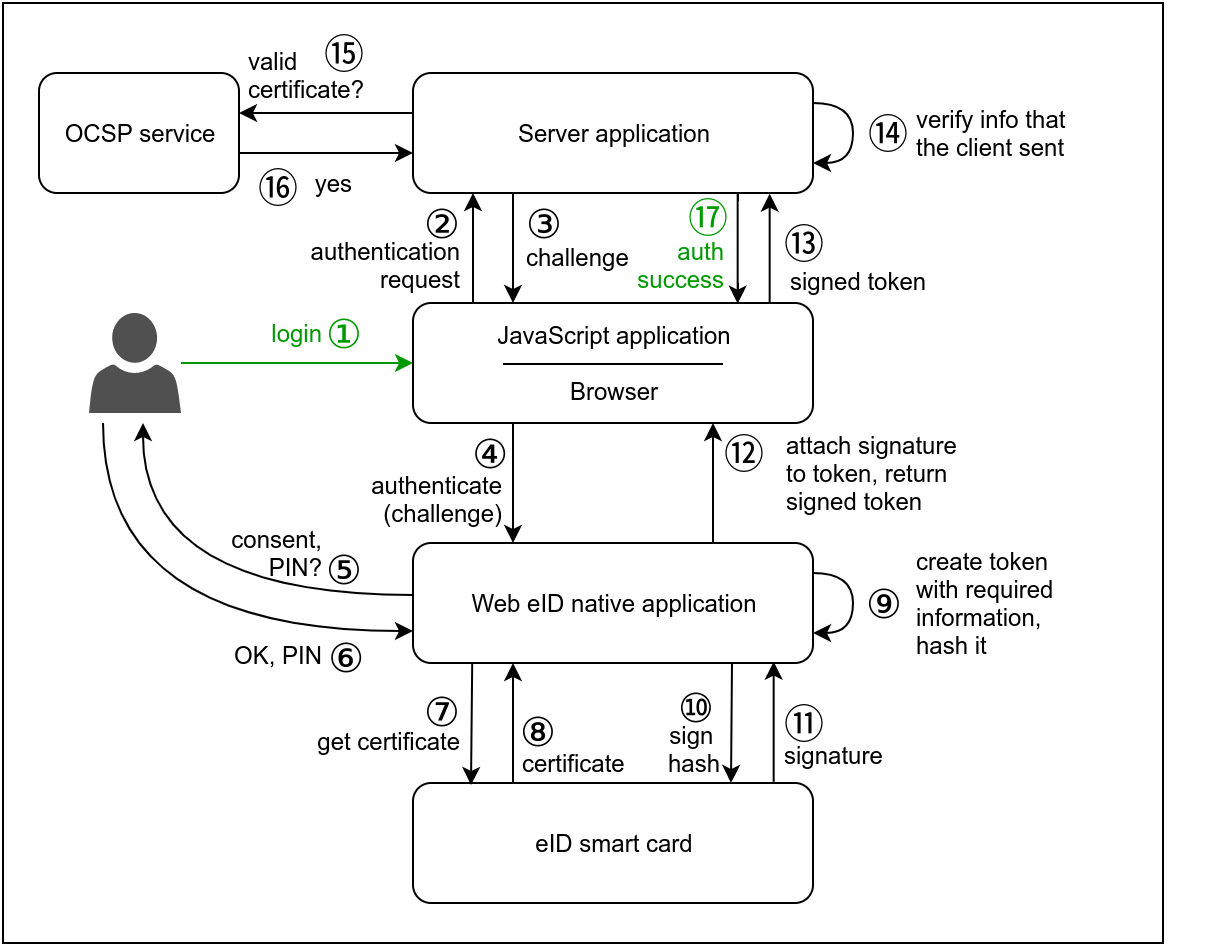
\includegraphics[width=\columnwidth]{img/authentication.png}
\caption{Web eID authentication diagram}\label{fig:auth}
\end{figure}

The eID authentication protocol is depicted in Figure~\ref{fig:auth}.

\subsection{Protocol model}\label{sec:authmodel}

\paragraph{Protocol parties:}

\begin{itemize}
\item User (U)   -- the user who wants to be authenticated;
\item Server (S) -- the server who authenticates;
\item Browser    -- the browser with JavaScript interpreter running in the user's local machine;
\item EID        -- Web eID native application running in the user's system;
\item SCard      -- smart card owned by the user;
\item Online Certificate Status Protocol (OCSP) service is not modeled as a separate party, and we assume that the Server has a black-box access to OCSP functionality.
\end{itemize}

\paragraph{Assumptions:}

We model a MITM attacker that intercepts communication in the public network. We ignore most of the possible internal threats such as learning the user's PIN or hacking into the OCSP service, which need to be treated separately. We only focus on threats coming from an external attacker. Denial-of-service attacks are also out of scope of ProVerif.

\begin{itemize}
\item The attacker intercepts network communication between the JS application and the Server. That is, we do not model interception on the level of the user's local machine.

\item The attacker may run an unbounded number of honest user and honest server sessions. He decides who communicates with whom in which order. He can himself control an unbounded number of malicious users and malicious servers.
    \begin{itemize}
    \item The attacker may control a user. To simplify modelling, the ProVerif code is written such that an attacker has issued a smart card for each malicious identity, and the corresponding certificate is recorded in the OCSP service. The attacker cannot obtain a card issued to an honest user.
    \item The attacker may control a server. TLS certificates are not strong, and the attacker can impersonate an honest server. We check whether obtaining a fake certificate is necessary for a particular attack.
     \end{itemize}

\item By default, the attacker has full control over the network (as it is usually modeled in ProVerif), and no one prevents him from getting all messages ever sent over transparent channels. To model the assumption that the attacker can only intercept the messages that are sent to his own IP addresses, we model DNS, which fixes an IP address for each identity, and creates a personal private channel for it. The attacker cannot read the messages destined to an honest party's IP unless it has been spoofed. We check whether DNS spoofing is necessary for a particular attack.

Alternatively, we could allow \emph{several} IP addresses for the same identity S. However, in our analysis, we assume that it is fine if the user connects to a different IP as far as the corresponding identity S is still correct. We also do not distinguish between the attacks related to adding a fake DNS record, or modifying an existing DNS record. Hence, we assume that one IP address per identity is sufficient.

%\item The EID service cannot be corrupted. Otherwise, the whole system would become insecure, as it would just learn the user's PIN and could do whatever if wants.

\item We assume that, once a TLS channel is established, it stays there until the end of authentication. We do not model the internal life of TLS and possible attacks on it. In practice, one should be careful with session resumption of TLS, as discussed in Sec~\ref{sec:mitm_risks_mitigations}.
\end{itemize}

\paragraph{Protocol steps:}We now describe the protocol steps in details. In the following, we use notation [$\cdot$] to denote optional values that are needed to be sent only for some settings.
\begin{enumerate}
\item\label{item:auth:step1} User inputs into browser the identity S of the server to connect with. Here the 'identity' is the same as the one stated in TLS certificate.
\begin{verbatim}
   U -> Browser: S
\end{verbatim}
\item\label{item:auth:step2} Browser makes a DNS lookup, finds the certificate of server S (which is potentially falsified), establishes TLS connection, and asks for a challenge
\begin{verbatim}
   Browser -TLS-> S: 'authRequest'
\end{verbatim}
\item\label{item:auth:step3} Server S generates a fresh nonce N and sends it to Browser. The message is marked as 'challenge', as N can be an arbitrary bitstring and has no special format. If we want to apply the protection method of Sec.~\ref{sec:challenge_signing}, we also require a signature NSign on N.
\begin{verbatim}
   S -TLS-> Browser: 'challenge', N, [NSign]
\end{verbatim}
\item\label{item:auth:step4} Browser sends to EID a request to meet the challenge. It also delivers the server hostname S, so that EID could display it to the user. If we choose to sign the server TLS certificate or the server's signature on challenge (i.e. apply protection profile of Sec.~\ref{sec:cert_validation} or Sec.~\ref{sec:challenge_signing}), we need to submit these as well.
\begin{verbatim}
   Browser -> EID: 'authRequest',S,N, [ServerCert, NSign]
\end{verbatim}
\item\label{item:auth:step5} EID prompts a PIN from User. In ProVerif model, we add S and N to the message, so that the inserted PIN can be linked to a particular authentication session. I.e. the response S,N,PIN cannot be used for another session S',N',PIN for S $\neq$ S' or N $\neq$ N'. In the next step, we discuss the necessity of actually displaying S and N to the user.
\begin{verbatim}
   EID -> User: S, N,'need_pin'
\end{verbatim}
\item\label{item:auth:step6} User inserts the PIN. EID application has to link the received PIN to the correct authentication session. In practice, if several sessions are running in parallel (e.g. another session is initiated by clicking on something by mistake), then the user should be aware of which session exactly he is approving. Ideally, we can display to the user the server identity S and the challenge N (or some other session ID derived from these two, e.g. a visual image) which he should verify against the values he sees in the 'correct' browser window. It may happen that a careless user does not perform this visual check, or there is some security environment that allows to re-use the PIN without user having to enter it again. In ProVerif model, we consider both possibilities, and we need to add S,N to the user's response if we want to link the inserted PIN to the correct session.
%User inserts the PIN. We assume that EID is able to link the received PIN with the correct S and N, and it is not possible to re-use the PIN. In our model, we consider also the case where the user does not perform a careful visual check before inserting the PIN, so adding S,N depends on this setting.
\begin{verbatim}
   User -> EID: PIN, [S,N]
\end{verbatim}
\item\label{item:auth:step7} EID gets the certificate out of the smart card.
\begin{verbatim}
   EID -> SCard: 'getCertificate()'
\end{verbatim}
\item\label{item:auth:step8} SCard returns the certificate UserCert to anyone who asks for it, without a PIN.
\begin{verbatim}
   SCard -> EID: UserCert
\end{verbatim}
\item\label{item:auth:step9} EID computes a token T = hash(T'), where T' depends on the protection profile. Let ServerCert be Server's TLS certificate (possibly fake) that has been chosen on User's side to establish TLS connection. The value of T' can be one of the following.

\begin{itemize}
\item hash(N) if no MITM protection methods are used.
\item hash(S,N) for the protection method of Sec.~\ref{sec:origin_validation}.
\item hash(S,N,ServerCert) for the protection method of Sec.~\ref{sec:cert_validation}. In a real application, the server certificate SHA-256 fingerprint is used instead of the full certificate. This does not make any difference to ProVerif model, as we do not model details of cryptographic primitives and treat all hashes as ideal.
\item hash(S,N,NSign) for the protection method of Sec.~\ref{sec:challenge_signing}. If we do not add NSign to the token, then the Server will not be able to check later whether the signature received by the User was correct, and MITM can sign N himself with his own TLS key.
\end{itemize}


\item\label{item:auth:step10} EID forwards the PIN to SCard and asks for a signature on T. A unique identifier SID links the output of SCard to a particular input to avoid messing up signatures of different messages. SID is a part of ProVerif model that is not explicitly generated in the real protocol. In practice, EID application should match the signature it receives from SCard to the appropriate authentication session,  even if several sessions are running in parallel.
\begin{verbatim}
   EID -> SCard: SID, T, PIN
\end{verbatim}
\item\label{item:auth:step11} The SCard computes the signature Sign = sign(SK,T) on T, where SK is the user's secret key stored in SCard, and sends it to EID.
\begin{verbatim}
   SCard -> EID: SID, Sign
\end{verbatim}
\item\label{item:auth:step12} EID attaches Sign to the token T and forwards these to Browser. EID also sends the user certificate UserCert, which can be later be verified against OCSP service.
\begin{verbatim}
   EID -> Browser: UserCert, T, Sign
\end{verbatim}
\item\label{item:auth:step13} Browser forwards received data to the Server through TLS pipe.
\begin{verbatim}
   Browser -TLS-> S: UserCert, T, Sign
\end{verbatim}
\item\label{item:auth:step14} The Server verifies the signature and the values stored in T.

\item\label{item:auth:step15} The Server consults the OCSP service whether the certificate is valid.

\item\label{item:auth:step16} The Server proceeds only of OCSP has approved the certificate.

\item\label{item:auth:step17} The Server notifies Browser that the authentication succeeded. The 'ok' message should be accompanied with the user name A and the nonce N for which the agreement has been established. These values prevent the attacker from replaying 'ok' message from some previous session. The user name A can be removed if TLS itself ensures that the message of S that is meant for Bob will not be accepted by Alice. In ProVerif models, we do not assume the latter by default, as the protocol works with transparent TLS, where no shared key has been established yet.
\begin{verbatim}
   Server -TLS-> Browser: A, N, 'ok'
\end{verbatim}
\item\label{item:auth:step18} The browser displays to the user a message 'ok'. This additional message is needed for modeling purpose, to verify the consistency of views of the User and the Server.
\begin{verbatim}
   Browser -> User: S, 'ok'
\end{verbatim}
\end{enumerate}

\subsection{Security analysis}

In the model, we consider relations between the following events.

\begin{itemize}
\item \texttt{event honest(A)} -- the secret key of party A is not known to the attacker.
\item \texttt{event honestPK(S,PK)} -- PK is the actual public key of the server S.

\item \texttt{event fakeServerCert(S)} -- attacker has obtained a fake TLS certificate of S.
\item \texttt{event dnsPoisonedName(S)} -- attacker modified the DNS table entry of the party S.
\item \texttt{event carelessUser(A)} -- the user ignores messages accompanying PIN request.

\item \texttt{event signedBySCard(A,M)} -- the smart card of party A has signed a message M.

\item \texttt{event beginUser(A,S)} -- the user A started establishing a session with S.
\item \texttt{event endUser(A,S)}   -- the user A has finished authentication to S.

\item \texttt{event endServer(A,S,N)} -- the server S has accepted authentication of A w.r.t. challenge N.
\item \texttt{event endJS(A,S,N,PK)} -- the JS interpreter at A's side has finished session with S w.r.t. challenge N, where PK is the public key of S used to establish TLS connection.

\item \texttt{event tlsJS(A,S,TlsNonce)} -- the JS interpreter at A's side established a TLS session defined by TlsNonce with S.
\item \texttt{event tlsServer(A,S,TlsNonce)}-- the server S established a TLS session defined by TlsNonce with JS interpreter at A's side.
\end{itemize}


We will further mark with '+' successful security proofs (ProVerif answers TRUE), and with '-' the disproofs (ProVerif answers FALSE, i.e. an attack trace is found). We group the ProVerif queries according to security goals. For each query, we first display the straightforward ProVerif statement, based on the events listed above, and then explain what it means.

In the following, we use the variable $T$ to denote the token signed by the user. The exact structure of this token depends on the protection profile. If the answer to the query turns out to depend on the choice of $T$, we mark it as $\pm$ and discuss it.

We are going to analyze whether an honest user A or an honest server S can be impersonated. We assume that an honest party always behaves according to the protocol rules, and we do not aim to protect a party that does not follow the protocol. A misbehaving party is treated as corrupted, and ProVerif does take into account the harm that it may cause to some other party. The attacker is allowed to control any number of servers and any number of users, so the model is not constrained to interactions between an honest user A and an honest server S.

\paragraph{Can attacker impersonate A to S?}

\begin{itemize}
\item[+] \texttt{query A : party, S : party, N : bitstring,\\
                 NSign : signature, PKS : pkey;\\
                 event(honest(A)) \&\& inj-event(endServer(A,S,N))\\
                 ==> inj-event(signedBySCard(A,$T$)).}

If the server S thinks that he established a connection with an honest user A with session nonce N, then indeed the smart card of A was used to sign the token $T$ of that session. This proves that authentication will not work without smart card signing the challenge. This does not yet prove that the user A is aware of what has been signed with their card.

\item[--] \texttt{query A : party, S : party, N : bitstring;\\
                  event(honest(A)) \&\& event(endServer(A,S,N))\\
                  ==> event(beginUser(A,S)).}

If the server S thinks that he established a connection with an honest user A with session nonce N, but the PIN is not linked to the server hostname, then it may be a replay attack where A actually does not intend to authenticate to S.

\item[$\pm$] \texttt{query A : party, S : party, N : bitstring;\\
                 event(honest(A)) \&\& inj-event(endServer(A,S,N))\\
                 ==> inj-event(beginUser(A,S)) || event(carelessUser(A)).}

If the server S thinks that he established a connection with an honest user A with session nonce N, then unless the user's PIN has been inserted into a wrong window, the user A has indeed wanted to connect to S. This fact depends on the used protection mechanism.
\begin{itemize}
\item[--] If no protection mechanisms are applied, then the response of A is not linked to any server identity, and the challenge N could have been forwarded by a MITM attacker.
\item[+] If we apply the protection method of Sec.~\ref{sec:origin_validation}, then the signature of A on the origin prevents server from accepting messages that A planned for some other origin.
\item[+] The method of Sec.~\ref{sec:cert_validation}   contains the origin as well, and works similarly to Sec.~\ref{sec:origin_validation}.
\item[+] The method of Sec.~\ref{sec:challenge_signing} contains the origin as well, and works similarly to Sec.~\ref{sec:origin_validation}.
\end{itemize}
If ProVerif answers TRUE to this query, the liveness of A is proven. However, this does not yet prove that A is indeed on the other end of the TLS pipe.

\item[$\pm$] \texttt{query A : party, S : party, TlsNonce : bitstring;\\
                 event(honest(A)) \&\& event(tlsServer(A,S,TlsNonce))\\
                 ==> event(tlsJS(A,S,TlsNonce)).}

If the server authenticates A, then A is indeed on the other end of TLS pipe. This fact depends on the used protection mechanism.
\begin{itemize}
\item[--] If no protection mechanisms are applied, then the response of A is not linked neither to any server identity nor any TLS pipe.
\item[$\pm$] If we apply the protection method of Sec.~\ref{sec:origin_validation}, then a MITM attacker that gets a fake certificate of S may forward the signed challenge of A to S through a separate TLS connection. For this, the attacker needs to intercept the message that A intended for S. If the attacker can intercept only those messages that are destined to an IP address controlled by it, then everything is fine as far as DNS table has not been poisoned (ProVerif will answer TRUE if we add \texttt{|| event(dnsPoisonedName(S))} or \texttt{|| event(fakeServerCert(S))} to the right-hand-side). In practice, we would still not be protected e.g. against malware that intercepts all outgoing messages, or an attacker located at the LAN gateway.
\item[+] If we apply the protection method of Sec.~\ref{sec:cert_validation}, then the signature of A on the certificate used in TLS prevents server from accepting a TLS connection that originates from an attacker. We assume that the Server and the Attacker do cannot share the same certificate, and there would still be an attack if the attacker managed to steal the private key corresponding to the TLS certificate owned by the Server.
\item[+] The protection method of Sec.~\ref{sec:challenge_signing} works similarly to the method of Sec.~\ref{sec:origin_validation}. Instead of signing the TLS certificate directly, A signs the signature on challenge that it received from S, which is indirectly linked to TLS certificate as well.
\end{itemize}

\end{itemize}

We conclude that, as far as the additional protection methods of Sec.~\ref{sec:protection_profiles} are applied, the server can be convinced that the user is alive, and indeed sits on the other end of the TLS pipe.

\paragraph{Can attacker impersonate S to A?}

\begin{itemize}

\item[--] \texttt{query A : party, S : party, PK : pkey, N : bitstring;\\
                  event(honest(S)) \&\& event(endJS(A,S,N,PK))\\
                  ==> event(endServer(A,S,N)).}

Without A checking the public key PK or the IP address of the server S against a trusted source, the attacker may easily impersonate S by presenting a fake TLS certificate.

\item[+] \texttt{query A : party, S : party, PK : pkey, N : bitstring;\\
                 event(honestPK(S,PK)) \&\& inj-event(endJS(A,S,N,PK))\\
                 ==> inj-event(endServer(A,S,N)).}

If the browser is convinced that the server's public key used in generation of TLS was indeed the honest server's one (e.g. confirmed using side-channels), then the nonce N was indeed generated by the server S that owns the corresponding secret key PK. So even though the user might not know which session exactly was accepted, the browser does know it.

\item[+] \texttt{query A : party, S : party, PK : pkey, N : bitstring;\\
                 event(honest(S)) \&\& inj-event(endJS(A,S,N,PK))\\
                 ==> inj-event(endServer(A,S,N)) || event(dnsPoisonedName(S)).}

If CA is not trusted, then the browser may instead read server's IP address from a trusted DNS table. This works as far as there is no DNS poisoning or message redirection.

\item[+] \texttt{query A : party, S : party, PK : pkey, N : bitstring;\\
                 event(honest(S)) \&\& event(endUser(A,S))\\
                 ==> event(endServer(A,S,N))|| event(fakeServerCert(S)).}

As far as the server has not been impersonated by fake certificates, the user that has received an authentication approval response can be sure that the real server approved at least one of the sessions that the user attempted to establish.

\item[--] \texttt{query A : party, S : party, PK : pkey, N : bitstring;\\
                 event(honest(S)) \&\& inj-event(endUser(A,S))\\
                 ==> inj-event(endServer(A,S,N)) || event(fakeServerCert(S)).}

Let us now see whether the \emph{injective} variant of the previous agreement query holds, i.e. is each server's acceptance is followed by \emph{at most one} user's acceptance. If there are several sessions running in parallel, the user may get a wrong opinion which one of them exactly was run with the true server S. This is because we do not show the nonce  to the user. This is not a problem, since it does not matter for the user which one of the sessions was accepted. From the previous queries, we see that the browser does know what the correct session ID is.

\end{itemize}

We conclude that the attacker cannot impersonate S unless he obtains at once a fake certificate and corrupts the DNS service. %Alternatively, if the server obtains an additional \emph{strong} certificate that cannot be faked, then it can use the corresponding key to sign the messages of steps (\ref{item:step3}) and (\ref{item:step17}), thus applying a variant of protection method described in Sec.~\ref{sec:challenge_signing}. Note that if the server signs \emph{only} the challenge at step (\ref{item:step3}), then a MITM attacker will stop forwarding messages to S and continues playing S to A, so signing (\ref{item:step17}) is important as well. It is also important that the additional signature is generated using a more trustworthy (or at least different) certificate, so that the attacker cannot just generate the additional signature of S himself.

\paragraph{Can the attacker misuse the smart card, which may potentially endanger other applications that use the same card?}

\begin{itemize}
\item[+] \texttt{query A : party, S : party, N : bitstring,\\
                 NSign : signature, PKS : pkey;\\
                 event(signedBySCard(A,$T$))\\
                 ==> event(beginUser(A,S,N)) || event(carelessUser(A)).}

If a smart card has signed something in scope of our protocol, then the user is aware of it, unless the PIN has been inserted into a wrong window. Note that the events are not injective, so if the user has approved signing a message M once, it does not yet mean that the same message can be signed multiple times without user being aware.

\item[--] \texttt{query A : party, S : party, N : bitstring,\\
                  NSign : signature, PKS : pkey;
                  event(honest(A))\&\& event(honest(S))\&\& inj-event(signedBySCard(A,$T$))\\
                  ==> inj-event(beginUser(A,S,N)) || event(carelessUser(A)).}

Let us now see whether the \emph{injective} variant of the previous agreement query holds, i.e. is each PIN insertion followed by \emph{at most one} signing. We see that, even if we link the user's PIN to a particular server hostname S and nonce N, it can be used multiple times to sign exactly the same message. This could potentially make some signature forging attacks easier by outputting signatures of the same message with different randomness. This issue seems more like ProVerif incompleteness than a real attack, as in reality an honest EID would prompt the PIN again each time, even if the message to be signed is exactly the same. ProVerif assumes that, once a message was sent to some channel, it can be used an unbounded number of times.
\end{itemize}

We conclude that generation of fake signatures is not possible without user being aware of that, as far as the PIN has been linked to the correct session.

\section{Signing Protocol}
\begin{figure}
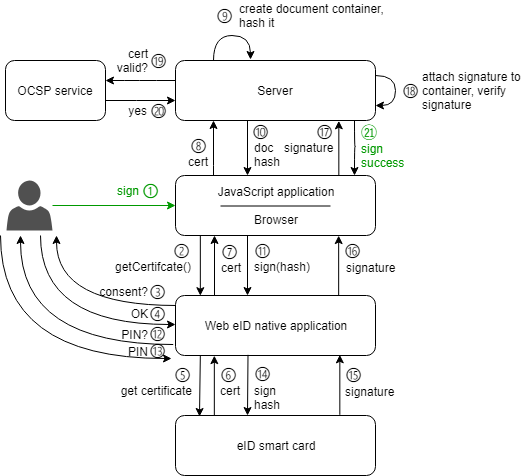
\includegraphics[width=\textwidth]{img/signing.png}
\caption{Web eID signing diagram}\label{fig:sign}
\end{figure}

The eID signing protocol is depicted in Figure~\ref{fig:sign}.

\subsection{Protocol model}

As the protocol structure is very similar to that authentication protocol, the set of parties and the assumptions are the same as in Sec.~\ref{sec:authmodel}.

\paragraph{Protocol steps:}

\begin{enumerate}
\item User inputs into Browser the identity S of the server to connect with. Here the 'identity' is the same as the one stated in TLS certificate. 
\begin{verbatim}
   U -> Browser: S
\end{verbatim}
\item Browser queries from EID the certificate by sending a constant message.
\begin{verbatim}
   Browser -> EID: 'getCertificate()'
\end{verbatim}
\item EID shows the constant message 'consent' to the user to verify their presence.
\begin{verbatim}
   EID -> U: 'consent'
\end{verbatim}
\item User confirms the consent. We note that the messages are not linked to particular S with which User tries to connect. Since the same certificate is used in all sessions, and it is public, this is not a problem.
\begin{verbatim}
   U -> EID: 'ok'
\end{verbatim}
\item EID gets the certificate out of the smart card.
\begin{verbatim}
   EID -> SCard: 'getCertificate()'
\end{verbatim}
\item SCard returns the certificate UserCert to anyone who asks for it, without a PIN.
\begin{verbatim}
   SCard -> EID: UserCert
\end{verbatim}
\item EID forwards UserCert to Browser.
\begin{verbatim}
   EID -> Browser: UserCert
\end{verbatim}
\item Browser makes a DNS lookup, finds the certificate of server S (which is potentially fake), establishes TLS connection, and sends UserCert to S.
\begin{verbatim}
   Browser -TLS-> Server: UserCert
\end{verbatim}
\item Server creates a document container and hashes it with a fresh randomness, creating a nonce N. At this point, server has not yet verified UserCert.

\item Server sends fresh randomness N to Browser. In reality, N would be a randomized document container, but we model it just as a random number. Including the randomness into document container is important to avoid replay attacks. If we want to apply the protection method of Sec.~\ref{sec:challenge_signing}, we also require a signature NSign on N.
\begin{verbatim}
   Server -TLS-> Browser: 'challenge',N, [NSign]
\end{verbatim}
\item Browser asks EID for a signature. We need to deliver the server identity S as well, as it will be displayed to the user. If we choose to sign one the server TLS certificate, or the server's signature on challenge, we need to submit these as well.
\begin{verbatim}
   Browser -> EID: 'authRequest',S,N, [ServerCert, NSign]
\end{verbatim}
\item EID prompts a PIN from the User. In ProVerif model, we add S and N to the message, so that the inserted PIN can be linked to a particular authentication session. I.e. the response S,N,PIN cannot be used for another session S',N',PIN for S $\neq$ S' or N $\neq$ N'.
%EID prompts a PIN from the User. It is important to display to the user the server name S, to avoid signing challenge of some other server. Displaying N does not help much, as it looks as a completely random value to the user anyway. Including N is important if the contents of the document container are important, and e.g. the user may decide to refuse to sign even an honest server's challenge. In ProVerif model, adding N to the message is needed for linking the PIN response to a particular authentication session. I.e. the response S,N,PIN cannot be used to generate a signature for another session S,N',PIN for N $\neq$ N'.
\begin{verbatim}
   EID -> User: S,N,'need_pin'
\end{verbatim}
\item User sends PIN to the EID application, which has to link it to the correct authentication session. Similarly to authentication protocol, we need to add S,N to the user's response if we want to link the inserted PIN to the correct session. Including N is more important for the signing protocol, since N depends on the contents of the document container, and the user should see what he is signing even if the server identity S is correct.
\begin{verbatim}
   User -> EID: PIN, [S,N]
\end{verbatim}
\item Similarly to the authentication protocol, EID constructs a token T according to particular protection profile, and a unique identifier SID links the output of SCard to a particular input to avoid messing up signatures of different messages.
\begin{verbatim}
   EID -> SCard: SID, T, PIN
\end{verbatim}
\item The SCard computes the signature Sign = sign(SK,T) on T, where SK is the user's secret key stored in SCard, and sends it to EID.
\begin{verbatim}
   SCard -> EID: SID, Sign
\end{verbatim}
\item EID forwards the signature Sign to Browser.
\begin{verbatim}
   EID -> Browser: Sign
\end{verbatim}
\item Browser forwards the signature Sign to the Server. We label this message as 'userSignature', since a signature itself is a bitstring which does not have a specific format, and can be confused with other messages.
\begin{verbatim}
   Browser -TLS-> S: 'userSignature', Sign
\end{verbatim}
\item The Server verifies the signature and attaches it to the container.

\item The Server consults the OCSP service whether the certificate is valid.

\item The Server proceeds only of OCSP has approved the certificate.

\item The Server notifies the Browser that the signing succeeded.
\begin{verbatim}
   Server -TLS-> Browser: A, N, 'ok'
\end{verbatim}
\item The browser displays to the user a message 'ok'. This additional message is needed mainly for modeling purpose, to verify the consistency of views of an honest User and an honest Server.
\begin{verbatim}
   Browser -> User: S, 'ok'
\end{verbatim}
\end{enumerate}

\subsection{Security analysis}

As the protocol structure is very similar to that of authentication protocol, we run the same ProVerif queries. The answers to these queries are similar to the authentication protocol, sharing same strengths and weaknesses. There are however some small differences.

\begin{itemize}

\item Signing the origin and/or the TLS certificate (protection profiles of Sec.~\ref{sec:origin_validation} and Sec.~\ref{sec:cert_validation}) help to prove that, if the server authenticates A, then A is indeed on the other end of TLS pipe. The advantage of signing protocol is that it finishes after the last step, so we do not need to worry what happens next, and whether A has indeed been on the other end of the TLS pipe. The goal of the protocol is still achieved as far as the real A signed the document that the server wanted it to sign, even if the MITM attacker forwarded all messages.

\item If the document container to be signed contains private information, then it may indeed be important who is on the other side of TLS. In this case, A would need to be authenticated \emph{before} the document container hash is sent out, which would be something different from the protocol of Fig.~\ref{fig:sign}.
\item
Differently from authentication, it can now be important to see which challenge N exactly was signed. That is, when the user inserts PIN, he sees the contents of the signed document container through the browser, and not through eID interface. While it is impractical to show the entire signed document through eID window, the value N is anyway not the document itself, but a hash, which could possibly be displayed by eID as well to reduce trust in browser. Again, since the user cannot compute the hash from visually observed document, they would need to trust the browser to do this automatically, or download the document and compute the hash by some independent tool, which would already make the ceremony very different from what we had initially. Visual verification of a hash can also be challenging, as small difference in some symbols can easily remain unnoticed.
\end{itemize}

\newcommand{\implies}{\Rightarrow}
\newcommand{\dns}{\mathsf{A_{IP}}}
\newcommand{\tls}{\mathsf{A_{CERT}}}
\section{Summary}

Table~\ref{table:proverifsummary} summarizes the capabilities of an external attacker for different protection profiles for both the authentication and the signing protocols. To make the representation more compact, we denote the event ``\emph{the attacker is able to intercept messages destined to the server}'' as $\dns$, and ``\emph{the attacker can obtain a fake TLS certificate}'' as $\tls$.

We note that we do not consider the problems related to the assumption that the user thoroughly reads the hash that he is going to sign, and compares it carefully against the hash of the actual document that he wanted to get signed. Problems on user side are out of scope of an external attacker analysis.

\begin{table}[ht]
\center
\begin{tabular}{| l | l | l |}
\hline
protection profile &  user impersonation & server impersonation                \\
\hline
none              & NOT OK               & $\neg\dns\vee\neg\tls\implies$OK \\
origin signing  (Sec.~\ref{sec:origin_validation})    & $\neg\dns\vee\neg\tls\implies$OK & $\neg\dns\vee\neg\tls\implies$OK \\
cert signing (Sec.~\ref{sec:cert_validation})       & OK                   & $\neg\dns\vee\neg\tls\implies$OK \\
challenge signing (Sec.~\ref{sec:challenge_signing}) & OK               & $\neg\dns\vee\neg\tls\implies$OK \\
\hline
\end{tabular}
\caption{Summary of ProVerif analysis for different protection profiles, where $\dns$ denotes that the attacker can poison DNS tables, and $\tls$ that the attacker can obtain a fake certificate for an honest server's name.}\label{table:proverifsummary}
\end{table}



\bibliographystyle{plain}
\bibliography{sections/webextensions}
\end{document}




